% =============================================================================
%  main.tex  --  "Rank Before You Merge" (generic two-column review draft)
%  Converted from drafts/paper_acmmm.md (8445 words, 9 sections, 5 tables,
%  3 figure placeholders). Prepared for author/supervisor review.
%
%  DISCIPLINE (do not violate when editing):
%   - Every NUMBER is copied verbatim from the markdown source. Do not change.
%   - Red-line wording (scoped claims, the locked cascade-gate quote, the GQA
%     single-full-statement, "robust default, not uniformly optimal") is
%     copied verbatim. Do not weaken.
%   - Internal repository / digest paths are not typeset. The "Source: *.md"
%     provenance lines of the markdown (work notes) are intentionally omitted.
%
%  FIGURES: four figures embedded from figs/ (all from measured data; no
%   proxy / schematic / placeholder remains). fig1.pdf = two audited OCRBench
%   cases with measured retained-unit masks for three selectors; fig2.pdf =
%   operational and matched-boundary full-split deltas;
%   fig3_token_survival.pdf = measured qualitative maps; fig3.pdf = measured
%   quantitative mechanism diagnostics.
%
%  PAGE BUDGET (hard cap: <=8 pp body + <=2 pp refs). Compression points already
%   applied are marked  % [COMPRESSED ...] ; further optional levers are marked
%   % [COMPRESS-OPTIONAL ...] for the user to apply if the actual compile runs
%   long (see README_compile.txt, "if it overflows").
% =============================================================================

\documentclass[sigconf,nonacm]{acmart}

% --- packages actually used in this file -------------------------------------
\usepackage{booktabs}     % \toprule \midrule \bottomrule (acmart also loads it)
\usepackage{multirow}     % Table 1 / Table 2 model-column row spans
\usepackage{algorithm}    % Algorithm 1 float
\usepackage{algorithmic}  % Algorithm 1 pseudocode
\usepackage{pifont}       % \ding{51}=check, \ding{55}=cross (replaces emoji)
\usepackage{graphicx}     % \includegraphics (figures), \fbox placeholders
\usepackage{url}          % \path{} for any path-like strings
\setlength{\emergencystretch}{1em} % avoid narrow-column overfull lines

% --- generic two-column review front matter ----------------------------------
\setcopyright{none}
% This draft is not tied to a journal or conference. Keep the robust acmart
% two-column typography while suppressing venue, DOI, copyright, and CCS blocks.
\settopmatter{printacmref=false, printccs=false, printfolios=true}
\renewcommand\footnotetextcopyrightpermission[1]{}
% Add the target venue's official metadata only after the venue is selected.

% --- CCS concepts (metadata only; regenerate via the ACM CCS tool if desired) -
\begin{CCSXML}
<ccs2012>
<concept>
<concept_id>10010147.10010257</concept_id>
<concept_desc>Computing methodologies~Machine learning</concept_desc>
<concept_significance>500</concept_significance>
</concept>
<concept>
<concept_id>10010147.10010375</concept_id>
<concept_desc>Computing methodologies~Computer vision</concept_desc>
<concept_significance>500</concept_significance>
</concept>
<concept>
<concept_id>10010147.10010172</concept_id>
<concept_desc>Computing methodologies~Natural language processing</concept_desc>
<concept_significance>300</concept_significance>
</concept>
</ccs2012>
\end{CCSXML}
\ccsdesc[500]{Computing methodologies~Machine learning}
\ccsdesc[500]{Computing methodologies~Computer vision}
\ccsdesc[300]{Computing methodologies~Natural language processing}

\keywords{visual token compression, vision-language models, training-free
  inference, multimodal foundation models, inference efficiency}

\title[Rank Before You Merge]{Rank Before You Merge: A Stage Law for Training-Free Visual Token
  Compression in Merger-Equipped Vision-Language Models}

\author{Zhengxing Yan}
\hypersetup{pdfauthor={Zhengxing Yan}}

% =============================================================================
\begin{document}

% -----------------------------------------------------------------------------
\begin{abstract}
Native spatial mergers reduce visual-token count before the language model, but
their interaction with token selection remains under-controlled. We compare
query-blind L2 ranking before and after the merger at matched budgets. The
operational RBM implementation (Qwen3-VL layer 8) leads matched Post-L2 on all
nine TextVQA, DocVQA, and OCRBench cells across three models. A separate
full-split Qwen3-VL control at the main-merger boundary reveals a
workload-conditioned stage effect: pre-final leads post by $+27.7$ pp on
TextVQA, $+4.6$ pp on DocVQA, and $+235$ OCRBench points, whereas post leads by
$5.6$ pp on GQA; all four paired contrasts remain significant after Holm
correction.

On Qwen3-VL, the merger weakly preserves unit ranks and disproportionately
demotes edge-rich document units; swapping the pre ranking into the post path
recovers pre accuracy with identical selected-unit identities. We turn this into
\textbf{Rank-Before-Merge (RBM)}, a minimal, training-free stage change with no
learned scorer or query input. The gains are against the matched L2-family post arm,
not a universal method ranking: query-conditioned FastV remains stronger on
several reference-grounded and object-centric settings. On full OCRBench under
the same HF eager harness and 4M-pixel cap, RBM scores 559 vs 413 on Qwen3-VL
and 382 vs 295 on Qwen2.5-VL. RBM is therefore an OCR-oriented default rather
than a universal winner. Six prespecified extensions do not improve over
their stronger constituents. At 25\% retention, compression is stage-neutral in
speed, increasing throughput by $68\%$ on Qwen3-VL and
$1.8$--$2.5\times$ on InternVL3.
\end{abstract}

\maketitle

% FIG 1 --- place the visual summary at the first available double-column top.
% Keeping this immediately after \maketitle makes the float land on page 2.
\begin{figure*}[t!]
  \centering
  
\includegraphics[width=\textwidth]{figs/fig1.pdf}
  \caption{\textbf{Three selectors retain different visual evidence.}
  Two audited OCRBench cases compare RBM, Post-L2, and FastV-k3 at the same
  $\kappa=25\%$ visual-token budget on Qwen3-VL-8B. Blue native-grid cells are
  the visual units retained by each method; the underlying input remains
  visible for direct spatial comparison. Vector checks and crosses report
  answer correctness against the printed ground truth. In both examples, RBM
  preserves the answer-bearing text and answers correctly, while Post-L2 and
  FastV-k3 do not. These cases illustrate the selection behavior; aggregate
  effects and uncertainty are reported in Figure~\ref{fig:fig2}.}
  \Description{Two OCRBench image rows compare retained visual units for RBM,
  Post-L2, and FastV-k3 at 25 percent retention. The first ground truth is
  A105-108 and the second is OCTOBER 1999. Blue grid cells identify units kept
  by each selector. RBM is correct in both rows, while Post-L2 and FastV-k3 are
  incorrect, as indicated by vector check and cross marks.}
  \label{fig:fig1}
\end{figure*}

% =============================================================================
\section{Introduction}\label{sec:intro}
% =============================================================================

\textbf{Multimodal inference cost is a visual-token problem.} Visual-language
models (VLMs) process images as hundreds to tens of thousands of visual tokens,
making quadratic attention and key-value memory major inference costs.
Visual-token compression is therefore central to efficient document
understanding, scene-text QA, and OCR. In merger-equipped architectures such as
Qwen-VL and InternVL3, $2\!\times\!2$ patch groups are first merged, while prior
work focuses mainly on which tokens to keep and how to score them. The selection
stage, before or after the native merger, is rarely isolated as a matched
variable. Prior work notes Qwen's native token reduction~\cite{bai2025qwen25vl}
and OCR degradation from post-encoder merging~\cite{islam2025adaptmerge,yang2024visionzip};
we directly test the boundary by scoring the same units with query-blind L2 on
merger-input (pre) or merger-output (post) features at the same per-image
budget.

\textbf{Minimal operationalization: Rank-Before-Merge (RBM).} Score each
merger-input unit, retain the top-$\kappa$, then merge only the survivors. RBM
uses no attention weights, training, or query input. Because merging is
per-unit, a fixed kept set receives the same native per-unit merger operation;
byte identity is verified on Qwen3-VL. RBM changes which units reach the merger.
We use this rule to expose the stage variable, not to claim scorer novelty
(\S\ref{sec:rbm}).

\textbf{What falls out of it --- a workload-conditioned stage law.} The
operational layer-8 RBM arm leads matched Post-L2 on the evaluated text-dense
splits across two Qwen generations; the direction replicates on InternVL3.
Separately, the full-split matched-boundary Qwen3-VL control significantly
favors pre-merger ranking on TextVQA, DocVQA, and OCRBench, but significantly
favors post-merger ranking on GQA (\S\ref{sec:experiments}).

\textbf{Why the stage matters.} On Qwen3-VL, the learned merger weakly preserves
unit ranks (Spearman $\rho=0.14$--$0.36$), disproportionately demotes high-edge
units on documents, and yields to a ranking-swap control: the post path recovers
pre accuracy with identical selected sets (Jaccard $=1.000$ in all four tested
cells). Thus, where tested byte-exactly, the
ranking rather than the forward path explains the gap (\S\ref{sec:mechanism}).
This matched-rule result is distinct from the query-conditioned FastV comparison:
FastV remains stronger on several scene-text/object-centric cells, so RBM is a
query-blind, OCR-preserving robust default, not a universal winner
(\S\ref{sec:fastv}).

\textbf{Contributions.}
First, Qwen3-VL diagnostics connect merger-induced rank reshaping and edge-rich
unit demotion to the selected set (\S\ref{sec:mechanism}). Second, a full-split
matched-boundary control establishes a workload-conditioned stage effect, with
opposite preferences for text-centric tasks and GQA (\S\ref{sec:experiments}).
Third, we evaluate minimal RBM across three models, map its trade-off against
FastV, and report six unsuccessful extensions (\S\ref{sec:fastv},
\S\ref{sec:negative}).

% =============================================================================
\section{Related Work}\label{sec:related}
% =============================================================================

\textbf{Token pruning and merging.} VLM compressors select or merge visual
tokens at encoder outputs or inside early LLM layers. FastV uses LLM attention
and is our query-conditioned baseline~\cite{chen2024fastv}; PyramidDrop prunes
progressively~\cite{xing2024pyramiddrop}. FasterVLM and SparseVLM accelerate or
condition pruning~\cite{zhang2024fastervlm,zhang2024sparsevlm}; PruMerge and
FitPrune use merging or learned importance
\cite{shang2024prumerge,ye2024fitprune}.
Other selectors use visual attention, graph propagation, diversity, or
text-guided cues
\cite{wang2024vtccls,jiang2025gprune,luan2025adaptprune,yu2026visiontrim,baek2026agilepruner,fang2026prunesid}.
These approaches motivate strong baselines but do not match selection on the
two sides of a frozen model's native merger under a shared query-blind scorer.

\textbf{Merger-aware compression.} ToMe and AdaptMerge introduce an additional
token-merging operation~\cite{bolya2023tome,islam2025adaptmerge}; learned
projectors such as TokenPacker alter the visual interface
\cite{li2024tokenpacker}. VisionZip's inspected Qwen2.5-VL path selects after
PatchMerger~\cite{yang2024visionzip}; AnchorPrune likewise operates after
Qwen2.5-VL's model-specific spatial processing~\cite{oh2026anchorprune}.
GlimpsePrune, VScan, TransPrune, and V2Drop provide complementary Qwen-family or
layer-evolution comparisons
\cite{zeng2025glimpseprune,zhang2025vscan,li2026transprune,chen2026v2drop}, but
not the matched native-merger boundary control studied here.

\textbf{Recent design space.} Hierarchical selection and set coverage broaden
ranking~\cite{sun2026hiloprune,ma2026apet,xu2026score}. Reconstruction,
functional sensitivity, and learned conditioning offer other objectives
\cite{du2026coin,kim2026zooprune,lee2026spare,wang2026metacompress,song2026evocomp,sun2026ifprune,zhu2026hawk}.
Other work varies token lifetime or aggregates discarded content
\cite{wang2026informationhorizon,chen2026alvts,li2026crisp,lei2026core,li2026aot,zhang2026hybrid};
document-specific studies emphasize that aggregate accuracy can conceal lost
textual evidence~\cite{choi2026docprune,liu2026provenance}. QuietPrune acts
inside the ViT~\cite{gao2026quietprune}; PixelPrune acts before it
\cite{wang2026pixelprune}. FastV and PyramidDrop act later inside the LLM. Our
narrower question is where to rank native merge units while
leaving the model and merger unchanged.

\textbf{Evaluation.} We use official scorer implementations from the
lmms-eval family~\cite{zhang2024lmmseval} and confine throughput comparisons to
one engine, consistent with protocol-sensitive efficiency evaluation
\cite{wang2025effivlmbench}.

% =============================================================================
\section{Method --- Rank-Before-Merge (RBM)}\label{sec:method}
% =============================================================================

\subsection{Models, mergers, and the stage axis}\label{sec:models}

We study three merger-equipped VLMs with two merger designs. Qwen3-VL-8B
and Qwen2.5-VL-7B use a learned PatchMerger~\cite{bai2025qwen3vl,bai2025qwen25vl};
InternVL3-8B uses pixel-shuffle downsampling~\cite{zhu2025internvl3}.
All are served in bf16, eager
attention, vLLM 0.19 (V1)~\cite{kwon2023vllm}, single A40 (46~GB), greedy
decoding. The shared
pipeline is: image $\to$ ViT patch tokens $\to$ native merger ($2\!\times\!2$
groups $\to$ one token) $\to$ language model. The Qwen merger is \emph{not} an
averaging pool: the four patch features of each $2\!\times\!2$ group are
concatenated and projected by a small learned MLP (LayerNorm $\to$ fc1 $\to$
GELU $\to$ fc2) to one unit vector; the lossy step is the four-to-one nonlinear
projection, so a kept unit's representation is a nonlinear function of its four
patches. We verified this against the served implementation on both Qwen
generations.

\textbf{The stage axis (the experimental variable).} The two arms share model,
token count, decoding, and a query-blind L2 magnitude rule, while evaluating
that rule on the native feature state available on each side of the merger:
\begin{itemize}
  \item \textbf{Pre-merger (RBM).} For each $2\!\times\!2$ unit, average the
    L2 norms of its four merger-input patch vectors, keep the top-$\kappa N$,
    and pass only the
    survivors through the unmodified native merger (and, for Qwen3-VL, each
    deepstack merger). The merger operates exactly as in the uncompressed model,
    on a subset of units.
  \item \textbf{Post stage (contrast).} Either score the $N$ \emph{merged} units
    on merger-\emph{output} features and keep the top-$\kappa N$ (the stage used
    by published compression methods for merger-equipped VLMs, including
    VisionZip's Qwen path), or --- the stronger, query-conditioned contrast ---
    prune inside the LLM by layer-2 attention (the FastV stage). The main
    matrix (Table~\ref{tab:tab1}) uses the post-merger-L2
    contrast from the same query-blind L2 family; the
    layer-2 FastV contrast is used only in Table~\ref{tab:tab3}.
\end{itemize}

\textbf{Budget definition.} Retention $\kappa$ is defined over \emph{merge
units} relative to each image's \textbf{own} full unit count, so two methods at
the same $\kappa$ feed the language model the same number of visual tokens per
image; we verify equality of the mean post-merger token count per benchmark
(\textbf{iso-token} control), so any accuracy difference is attributable to
\emph{which} units survive and the representational state on which selection is
made, not to token count. We report $\kappa \in \{0.25, 0.125\}$ (25\% / 12.5\%
retention); per-benchmark token counts are printed with each table.

\subsection{The L2 selector as a control variable}\label{sec:selector}

We deliberately use the simplest \textbf{text-agnostic, query-blind}
L2-magnitude family. For unit $u$ with four merger-input patch vectors
$h_{u,1:4}$ and native merger $M$, the implemented scores are
\[
s_{\mathrm{pre}}(u)=\tfrac14\sum_{j=1}^{4}\|h_{u,j}\|_2,
\qquad
s_{\mathrm{post}}(u)=\|M(h_{u,1:4})\|_2.
\]
Thus the ranking functional is matched at the level of feature magnitude,
while its representation is the experimental stage: four input vectors before
the nonlinear merger versus its output vector after it. For Qwen3-VL, the
headline operational pre arm takes $h$ from the first deepstack tap (ViT
layer~8), whereas the matched-depth pre-final control takes $h$ from the final
ViT block at the main-merger boundary (\S\ref{sec:qwen}). We freeze plain RBM
and add no deployed variant. \S\ref{sec:mechanism} additionally
reports a mechanism-side probe: a \emph{variance-weighted} variant of the same
query-blind scorer, $s_{\text{freq}}(u) = \alpha\,z{}\!\left(\|f_u\|_2\right) +
\beta\,z{}\!\left(\mathrm{Var}_{u}\right)$ (both terms per-image standardized,
so the ratio $\alpha{:}\beta$ is a genuine trade-off knob rather than an
arbitrary scale), improves text-dense accuracy under aggressive compression
($+1.2$~pp TextVQA at 25\% retention, $+0.5$~pp at 50\%) yet is not a general
upgrade: it regresses $-1.6$ to $-2.2$~pp on DocVQA, OCR-Bench, and GQA at 25\%.
We therefore treat it as supporting evidence for \S\ref{sec:m2}'s
high-frequency-unit hypothesis rather than as a deployed selector variant
(\S\ref{sec:negative}). \S\ref{sec:modes} reports that the tested effect
survives replacing L2 with a second scorer family (global-centroid attention) on
Qwen3-VL, indicating the effect is not specific to L2. Unlike the merging
lineage of \S\ref{sec:related}, RBM introduces no second learned merger and no
query input: it manipulates only the \emph{set} of units the native merger sees
--- which is exactly what makes the pre-vs-post contrast a clean stage
experiment rather than a scorer comparison.

\subsection{Rank-Before-Merge}\label{sec:rbm}

Given an image with $N$ merge units, compute $s(u)$ on merger-input features for
every unit, retain the top $k = \kappa N$, and invoke the native merger(s) on
the retained units only. Unit identity is shared across the main and deepstack
streams (deepstack mergers process intermediate-depth features of the
\emph{same} units), so pruning a unit removes it from every stream. No attention
weights are required and no parameters are trained.

\textbf{Unit equivalence (the structural invariant).} Because the mask is at
\emph{unit} granularity and the merger is per-unit, a fixed kept set supplies
the same four patches to the same native per-unit operation. Selection cannot
prevent intra-unit combination; it changes which units reach the merger. The
resulting outputs are byte-identical in the verified Qwen3-VL path; other
families are limited to the evidence stated in \S\ref{sec:discussion}. Pre-merger
selection keeps units on their raw (merger-input) saliency; post-stage selection
keeps them on a saliency the merger has already rewritten (\S\ref{sec:mechanism}).
This invariant enables the ranking-swap control of \S\ref{sec:m3}.

\begin{algorithm}[t]
  \caption{Rank-Before-Merge (RBM), one image}
  \label{alg:rbm}
  \begin{algorithmic}[1]
    \REQUIRE image $x$; retention $\kappa$; query-blind scorer $s = \|\cdot\|_2$
    \ENSURE compressed visual token sequence $z$
    \STATE $P \gets$ ViT patch tokens of $x$ \COMMENT{16~px footprint}
    \STATE $U \gets$ group $P$ into $N$ native $2\!\times\!2$ units \COMMENT{32~px footprint}
    \FOR{each unit $u \in U$}
    \STATE $\mathrm{score}[u] \gets \frac14\sum_{j=1}^{4}\|h_{u,j}\|_2$ \COMMENT{mean patch L2}
    \ENDFOR
    \STATE $k \gets \max(1,\mathrm{round}(\kappa N));\ K \gets \mathrm{topk}(\mathrm{score},k)$
    \STATE $z_{\mathrm{main}} \gets \mathrm{NativeMerger}(\{u : u \in K\})$ \COMMENT{merge survivors only}
    \STATE $z_{\mathrm{ds}} \gets \mathrm{DeepstackMergers}(\{u : u \in K\})$ \COMMENT{Qwen3-VL only}
    \STATE $z \gets \mathrm{NativeVisualInterface}(z_{\mathrm{main}}, z_{\mathrm{ds}})$
    \RETURN $z$ \COMMENT{feed standard LLM}
  \end{algorithmic}
\end{algorithm}

\noindent\textbf{Post-merger selection (the contrast):} replace lines~3--5 of
Algorithm~\ref{alg:rbm} by $U' \gets \mathrm{NativeMerger}(U)$;
$\mathrm{score}'[u'] \gets \| f_{\mathrm{out}}(u') \|_2$ on merger-\emph{output}
features; $K' \gets$ top-$k$ by $\mathrm{score}'$; $\mathrm{keep}(K')$.
Everything downstream is identical.

% [COMPRESSED -> supp S8] The markdown's "Configuration disclosures" paragraph
% (the Qwen2.5-VL block-vs-interleaved M-RoPE position-cursor fix, and the
% per-family merger tap points) is condensed to one cross-reference here; the
% full detail lives in Supplementary S8.
\textbf{Configuration details.} Per-family tap points (Qwen3-VL
deepstack[0] at ViT layer~8, Qwen2.5-VL main merger input, InternVL3
pixel-shuffle input) and
the Qwen2.5-VL position-cursor fix are detailed in Supplementary~\S\,S8,
including the cross-generation configuration diagnostic.

% =============================================================================
\section{Main Experiments}\label{sec:experiments}
% =============================================================================

\subsection{Setup}\label{sec:setup}

\textbf{Benchmarks and metrics.} We use TextVQA VQA accuracy
~\cite{singh2019textvqa}, DocVQA ANLS~\cite{mathew2021docvqa}, the official
OCR-Bench score~\cite{liu2024ocrbench}, and GQA normalized exact
match~\cite{hudson2019gqa}. Official split sizes are 5000, 5349, 1000, and
12578, respectively. Scorers
are verbatim ports of the lmms-eval family~\cite{zhang2024lmmseval}, with
ground-truth self-test passing 200/200.

\textbf{Engines and fairness protocol.} RBM and the none / post cells run in
vLLM; the FastV baseline runs in an independent HuggingFace transformers eager
harness (it has no vLLM path). Accuracy is comparable across engines (the harness
bit-degrades to native at zero drop, 8/8 per-sample identical; HF-vs-vLLM none
cells agree 16/16); \textbf{throughput is not} --- all efficiency numbers are
confined to vLLM (\S\ref{sec:efficiency}). Fairness is enforced by the same keep
ratio relative to each image's own token count and by reporting mean
post-merger token counts.

\textbf{Significance.} Each pre-vs-post $\Delta$ pairs the same samples under
greedy decoding. The prespecified primary family comprises the nine
model$\times$text-dense-benchmark pre-vs-post contrasts at 25\% retention in
Table~\ref{tab:tab1}. We use 20,000-resample paired-bootstrap confidence
intervals on per-item metric differences and two-sided paired sign-flip
permutation tests; Holm correction across these nine tests gives
$p_{\mathrm{Holm}}\leq4.5\times10^{-4}$ for every contrast. McNemar is reported
only as a binary-outcome cross-check for OCRBench containment and GQA exact
match. Other budgets, GQA, mechanism probes, FastV comparisons, and extension
gates are secondary or exploratory and are not pooled into the primary family.
The metric-level tests preserve partial credit in VQA accuracy and ANLS rather
than binarizing those metrics. The four full-split matched-boundary contrasts
form a separate prespecified family; all remain significant after Holm
correction within that family.

\subsection{Main result across three models --- official full splits (Table 1)}\label{sec:qwen}

% --- TABLE 1 : wide (8 columns) -> table* spanning both columns ---------------
\begin{table*}[t!]
  \centering
  \small
  \caption{Operational RBM versus matched Post-L2 on official full splits
    ($n = 5000 / 5349 / 1000 / 12578$). $\Delta_{25}=$ RBM $-$ post at
    $\kappa=0.25$. Qwen3-VL RBM ranks at the layer-8 deepstack tap; this table
    is therefore an operational comparison, distinct from the matched-boundary
    control in Table~\ref{tab:matched_boundary}. Within each row the two arms
    use equal token budgets; full protocol and skip accounting are in the
    supplementary material.}
  \label{tab:tab1}
  \begin{tabular}{@{}ll r r r l r r@{}}
    \toprule
    Model & Benchmark (metric) & none & RBM @25\% & post @25\% & $\Delta_{25}$ & RBM @12.5\% & post @12.5\% \\
    \midrule
    \multirow{4}{*}{Qwen3-VL-8B}
      & TextVQA (VQA-acc)   & 0.844 & \textbf{0.605} & 0.222 & \textbf{+38.4 pp} & 0.472 & 0.132 \\
      & DocVQA (ANLS)       & 0.956 & \textbf{0.481} & 0.238 & \textbf{+24.3 pp} & 0.352 & 0.103 \\
      & OCR-Bench (/1000)   & 760   & \textbf{547}   & 184   & \textbf{+363 pts} & 350   & 53 \\
      & GQA (exact match)   & 0.616 & 0.449          & 0.477 & $-2.8$~pp \dag & ---   & --- \\
    \midrule
    \multirow{4}{*}{Qwen2.5-VL-7B}
      & TextVQA (VQA-acc)   & 0.862 & \textbf{0.702} & 0.442 & \textbf{+26.1 pp} & 0.597 & 0.319 \\
      & DocVQA (ANLS)       & 0.949 & \textbf{0.636} & 0.526 & \textbf{+11.0 pp} & 0.455 & 0.245 \\
      & OCR-Bench (/1000)   & 817   & \textbf{480}   & 182   & \textbf{+298 pts} & 328   & 70 \\
      & GQA (exact match)   & 0.604 & 0.559          & 0.585 & $-2.6$~pp \dag & ---   & --- \\
    \midrule
    \multirow{4}{*}{InternVL3-8B}
      & TextVQA (VQA-acc)   & 0.8338 & \textbf{0.7890} & 0.4148 & \textbf{+37.4 pp} & 0.7230 & 0.3064 \\
      & DocVQA (ANLS)       & 0.9221 & \textbf{0.7284} & 0.3820 & \textbf{+34.6 pp} & 0.5054 & 0.2451 \\
      & OCR-Bench (/1000)   & 852    & \textbf{753}    & 321    & \textbf{+432 pts} & ---    & --- \\
      & GQA (exact match)   & 0.6293 & 0.5993          & 0.6031 & $-0.4$ pp (n.s.)  & ---    & --- \\
    \bottomrule
  \end{tabular}

  \vspace{2pt}\footnotesize
  \textbf{Notes.} Qwen2.5-VL OCRBench uses the same 4M-pixel cap in both arms;
  mean effective prompt lengths are equal at each budget (229.6 at 25\%, 131.5
  at 12.5\%). InternVL3 uses pixel-shuffle and family-specific imaging; compare
  within-model deltas. Detailed configuration, inference, and skips are in the
  supplementary material.

  \vspace{2pt}
  \begin{minipage}{0.72\textwidth}
    \centering\small
    \captionof{table}{Qwen3-VL full-split matched-boundary control. $\Delta=$
    pre-final $-$ post; OCRBench differences and CIs are shown in /1000 points.}
    \label{tab:matched_boundary}
    \setlength{\tabcolsep}{3.2pt}
    \begin{tabular}{@{}lrrrrr@{}}
      \toprule
      Benchmark & pre-final & post & $\Delta$ & 95\% CI & $n$ \\
      \midrule
      TextVQA & .4985 & .2217 & $+27.68$ pp & $[+26.21,+29.19]$ & 5000 \\
      DocVQA & .2836 & .2377 & $+4.59$ pp & $[+3.43,+5.78]$ & 5349 \\
      OCRBench & 419 & 184 & $+235$ pt & $[+199,+271]$ & 1000 \\
      GQA & .4207 & .4771 & $-5.64$ pp & $[-6.42,-4.86]$ & 12578 \\
      \bottomrule
    \end{tabular}
    \par\vspace{2pt}\footnotesize Equal per-sample token counts; zero skips in both
    arms. All four paired tests remain significant after within-family Holm
    correction; full statistics are in Supplementary~S7b.
  \end{minipage}
\end{table*}

\textbf{Operational results.} Every text-dense
$\Delta_{25}$ is large and significant: RBM leads post-merger selection by
$+38.4$~pp (TextVQA), $+24.3$~pp (DocVQA), $+363$~pts (OCR-Bench; 547 vs 184,
$3.0\times$) on Qwen3-VL, and by $+26.1$~pp, $+11.0$~pp, and $+298$~points
(480 vs 182) on Qwen2.5-VL; all paired-bootstrap 95\% CIs exclude zero. The
matched-cap Qwen2.5-VL OCRBench values are 480 vs 182 ($+298$ points) at 25\%
and 328 vs 70 ($+258$ points) at 12.5\%. The gap is robust to
deeper compression: at $\kappa = 0.125$ the post stage degrades much faster
(Qwen3-VL OCR-Bench $184 \to 53$ vs RBM $547 \to 350$, widening the pre/post
ratio from $3.0\times$ to $6.6\times$), and all six text-dense $\Delta_{12.5}$
remain significant under paired metric-level inference.

\textbf{Full-split matched-boundary control.} Operational Qwen3-VL RBM ranks at
the layer-8 \texttt{deepstack[0]} input. To isolate the main-merger boundary,
pre-final instead ranks final ViT-block features immediately before that merger,
while post ranks its output. Both arms use $\kappa=0.25$, identical per-sample
token counts, greedy decoding, and zero skips.

The control reveals a workload-conditioned stage effect: text-, document-, and
OCR-centric tasks favor pre-merger ranking, whereas GQA significantly favors
post-merger ranking. Operational layer-8 RBM improves GQA over pre-final
(.4488 vs .4207) but remains below post (.4771), so neither operational nor
matched-boundary evidence supports a universal pre-merger advantage. The
no-merger LLaVA-1.5 control is summarized in Supplementary~S7c.

\begin{figure*}[t!]
  \centering
  
\includegraphics[width=\textwidth]{figs/fig2.pdf}
  \caption{\textbf{Operational and matched-boundary stage effects.}
  \textbf{(a)} Operational RBM minus Post-L2 on full splits; Qwen3-VL uses its
  layer-8 RBM tap. \textbf{(b)} The separate Qwen3-VL control ranks immediately
  before versus after the main merger. Whiskers are paired-bootstrap 95\% CIs;
  OCRBench /1000 differences are divided by 10. The matched control favors pre
  on text-centric workloads and post on GQA.}
  \Description{Two forest plots separate the operational cross-model comparison
  from the Qwen3-VL matched-boundary comparison. TextVQA, DocVQA, and OCRBench
  favor pre-merger ranking; matched-boundary GQA favors post-merger ranking.}
  \label{fig:fig2}
\end{figure*}

\subsection{Replication on a third family --- InternVL3-8B (Table 1)}\label{sec:internvl}

To test whether the Qwen direction replicates beyond that family, we run RBM
and the post stage on \textbf{InternVL3-8B},
whose merger is pixel-shuffle downsampling --- a different design from Qwen's
PatchMerger. The post arm here is \textbf{post-merger L2 top-k} --- the
same query-blind L2-magnitude family as the pre arm, at an identical
token budget (ptid equal across arms), so the InternVL3 block of
Table~\ref{tab:tab1} isolates the before/after merger stage under iso-budget
control at 25\% retention. The query-conditioned in-layer FastV contrast is a separate campaign,
reported in Table~\ref{tab:tab3}.

\textbf{Configuration boundary.} InternVL3 DocVQA uses a 4~M-pixel cap, while
the Qwen same-scope baseline cells of \S\ref{sec:fastv} use 600k; cross-model
absolute values are not comparable. At 25\% retention RBM costs $-19.4$~pp vs
none on InternVL3 DocVQA and $-99$/1000 on OCR-Bench, versus only $-4.5$~pp on
TextVQA and $-3.0$~pp on GQA. The claim is therefore the large within-model
pre$>$post margin, not losslessness on every text-dense workload.

At 12.5\% retention ($r=0.875$), TextVQA is 0.7230 pre
vs post 0.3064 (\textbf{+41.7 pp}); DocVQA pre 0.5054 vs post 0.2451
(\textbf{+26.0 pp}) --- the gap \emph{widens} under deeper compression, as on
Qwen.

\textbf{Cross-family directional replication.} InternVL3's pre$-$post text-dense gaps
($+37.4 / +34.6$~pp / $+432$~pts) are the same order and direction as
Qwen3-VL's ($+38.4 / +24.3 / +363$~pts) on all three text-dense benchmarks, and
GQA stays within the red line --- indistinguishable here ($-0.4$~pp), whereas
Qwen3-VL's matched-boundary control significantly favors post by $5.6$~pp
(\S\ref{sec:qwen}), with no
text-dense crossover at either family's native imaging configuration. These
accuracy-level replications show that the shared L2-magnitude rule can favor
the pre-merger side on a third model family with a different merger. They support
--- but do not by themselves establish --- the Qwen3-VL selection-level
mechanism as a cross-family explanation.

\textbf{The ranking-swap comparison on InternVL3.} The M3-style control
(\S\ref{sec:mechanism}) --- run the post-merger forward path but select units
with the pre-merger ranking --- closely matches pre-merger accuracy on the
three tested InternVL3 cells: swap vs pre is $+0.00$~pp (TextVQA), $+0.11$~pp
(DocVQA), and $-0.50$~pp (GQA), with kept-set Jaccard(pre,swap)$= 1.0$ and
per-sample answer-identity $0.98$--$1.0$ ($n=200$, iso-token, no swap
fallback). This supports a ranking-level explanation on a second merger
architecture (pixel-shuffle, not just Qwen's PatchMerger), but the nonzero
residuals mean that the byte-exact causal attribution remains specific to
Qwen3-VL.

\subsection{A workload-conditioned regime map --- RBM vs the query-conditioned strong baseline FastV (Table 2)}\label{sec:fastv}

FastV is the query-conditioned strong baseline in this comparison: it selects
inside the LLM after cross-attention has mixed in the question. We compare RBM
against the best tested FastV layer ($K=3$), with paired samples and official
rescoring within each row. We read
the result as a \textbf{workload-conditioned regime map} --- where
query-conditioned selection wins, where it fails, and why --- not as a
single-winner race. At its canonical progressive schedule
PyramidDrop is near-lossless but occupies a different budget point (equivalent
mean retention $0.625 \approx 2.1\times$ ours); at the tested iso-25\%
schedule it degrades sharply (TextVQA 0.073 / GQA 0.305 / OCR 0.005 on Qwen3-VL),
whereas RBM holds (0.60 / 0.42 / 0.58). There is therefore no universal winner.

\begin{table}[t]
  \centering
  \small
  \setlength{\tabcolsep}{2pt}
  \caption{Workload-conditioned comparison of
    FastV at best $K = 3$ (the query-conditioned strong baseline) vs RBM (pre,
    the query-blind OCR-oriented default) at 25\% retention. Configuration is
    matched within each row; scope and pixel cap are printed explicitly.}
  \label{tab:tab3}
  \begin{tabular}{@{}l r r r l@{}}
    \toprule
    Benchmark (scope; pixel cap) & $n$ & FastV-k3 & RBM @25\% & $\Delta$ (F/R) \\
    \midrule
    \multicolumn{5}{@{}l}{\textbf{Qwen3-VL-8B}} \\
    TextVQA (full; default)      & 5000  & \textbf{0.7771} & 0.605  & \textbf{+17.2 F} \\
    GQA (full; default)          & 12578 & \textbf{0.5376} & 0.449  & \textbf{+8.9 F} \\
    DocVQA (dev; 600k cap)       & 200   & \textbf{0.5863} & 0.4239 & \textbf{+16.2 F} \\
    OCR-Bench (full; 4M cap)     & 1000  & 0.413           & \textbf{0.559} & \textbf{+14.6 R} \\
    \midrule
    \multicolumn{5}{@{}l}{\textbf{Qwen2.5-VL-7B}} \\
    TextVQA (dev; default)       & 200   & \textbf{0.7467} & 0.6683 & \textbf{+7.8 F} \\
    GQA (dev; default)           & 200   & 0.475           & 0.520 & $+4.5$ R$^{\ddagger}$ \\
    DocVQA (dev; 600k cap)       & 200   & 0.4852          & 0.5062 & $+2.1$ R$^{\ddagger}$ \\
    OCR-Bench (full; 4M cap)     & 1000  & 0.295           & \textbf{0.382} & \textbf{+8.7 R} \\
    \bottomrule
  \end{tabular}

  \vspace{2pt}\footnotesize
  \textbf{Notes.} F = FastV; R = RBM. Only the OCRBench rows use the full
  1000-example, 4M-cap, HF eager control: symmetric skips are 79 (Qwen3-VL) and
  88 (Qwen2.5-VL), leaving paired answered sets of 921 and 912 for inference.
  Skips are identical across methods and cannot favor either arm. Other rows
  retain their printed full/dev scopes and configurations. $^{\ddagger}$The
  paired 95\% CI crosses zero; full harness, budget, and skip details are in the
  supplementary material.
\end{table}

\textbf{Workload-conditioned comparison.} FastV-k3 leads RBM on the three
Qwen3-VL non-OCR rows ($+17.2/+8.9/+16.2$ pp) and Qwen2.5-VL TextVQA
($+7.8$ pp), showing the value of question-conditioned selection. Conversely,
on full OCRBench RBM leads by 146/87 points on the /1000 scale; paired inference
uses only the 921/912 samples answered by both methods. The Qwen2.5-VL
$n=200$ GQA/DocVQA differences remain inconclusive. Thus later query
conditioning does not recover RBM's OCR accuracy under the tested control,
while it is beneficial on several non-OCR workloads.

% =============================================================================
\section{Mechanism --- How the Native Merger Reshapes Saliency Rankings}\label{sec:mechanism}
% =============================================================================

We give the pre-vs-post gap a mechanistic account in three parts (M1--M3),
measured on \textbf{Qwen3-VL-8B} (M1/M2 on a deterministic seed-0 $n = 64$ sample
per benchmark; M3 on $n = 200$ with the same invocation as the headline cells),
then state its architectural scope.

\subsection{M1 --- the merger reshuffles unit ranks}\label{sec:m1}

% [COMPRESSED -> supp S1] The markdown restated the rho / Jaccard ordering in
% two near-identical paragraphs; merged into one here. The full M1 table
% (Spearman rho, Kendall tau, Jaccard@25%) is Supplementary Table S1. All
% numbers are retained; the "source: ... snapshot draft" work-note is dropped.
Per image we correlate the \emph{pre} ranking (merger-input unit L2) with the
\emph{post} ranking (merged-token L2) over all units. The two rankings are
barely related, and the reshuffle tracks text density: Spearman
$\rho = \mathbf{0.137}$ (DocVQA, text-dense document) $< 0.332$ (TextVQA,
text-dense scene) $< \mathbf{0.360}$ (GQA, object-centric), with the
decision-relevant top-25\% overlap rising in the same order (Jaccard@25\%
$= 0.180 < 0.243 < 0.278$; full values in Supplementary~S1). The merger's
nonlinear projection thus reorders unit saliency almost from scratch
($\rho = 0.14$--$0.36$, nowhere near 1): both the full-ranking correlation and
the decision-relevant top-25\% overlap rise from the most text-dense benchmark
to the object-centric one, so the reshuffle is largest on DocVQA and smallest on
GQA --- yet substantial on every benchmark.

\subsection{M2 --- demoted units are disproportionately edge-rich}\label{sec:m2}

With rank\_shift $=$ post\_rank $-$ pre\_rank ($+$ $\Rightarrow$ demoted) and
per-unit Sobel edge energy as a high-frequency proxy, high-edge units are
disproportionately demoted at $\kappa=25\%$. The rank-shift/edge correlations
are $+0.439$ on DocVQA, $+0.155$ on TextVQA, and $+0.036$ on GQA ---
${\sim}12\times$ stronger on documents than on object scenes. Units post drops
that pre keeps are the highest-edge group: on DocVQA, mean Sobel
\textbf{0.641 vs 0.124} for the reverse group, with \textbf{92\% above the
per-image median (vs 35\%)}. This is consistent with demotion of structures
needed by text-centric recognition, but Sobel energy is not a text-region mask.
The full M2 table
(per-benchmark Sobel means and median fractions) is in Supplementary~S2.

\begin{figure*}[t!]
  \centering
  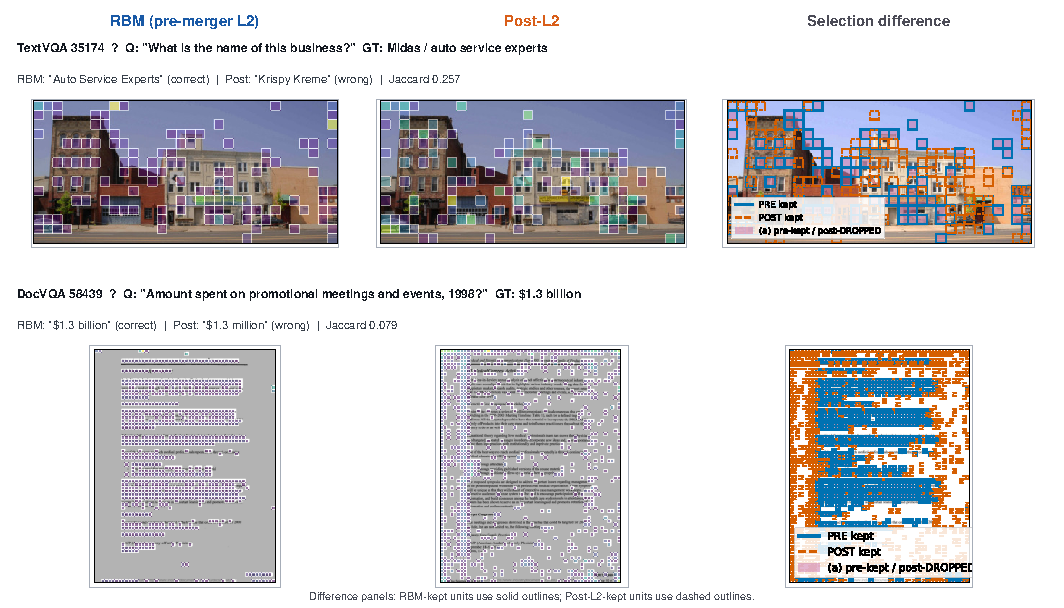
\includegraphics[width=0.90\textwidth]{figs/fig3_token_survival.pdf}
  \caption{\textbf{Measured token-survival maps at 25\% retention.} Rows show
  representative TextVQA and DocVQA examples; columns show units retained by
  operational RBM, Post-L2, and their selection difference. RBM preserves the
  correct answer in both cases, whereas Post-L2 does not. The maps reuse the
  recorded masks and predictions; they are qualitative examples, not aggregate
  accuracy evidence.}
  \Description{Two rows of visual-token maps compare RBM, Post-L2, and their
  selection difference on one TextVQA and one DocVQA example.}
  \label{fig:token_survival}
\end{figure*}

\subsection{M3 --- ranking-swap control with fixed token identities}\label{sec:m3}

By unit equivalence (\S\ref{sec:rbm}), holding the \emph{forward path} fixed at
post and swapping in the \emph{pre ranking} must reproduce pre accuracy if the
gap is purely a ranking effect. It does:

Swapping in the pre ranking recovers full pre-merger accuracy (exactly on
DocVQA; within 2/200 greedy-decode answers on TextVQA, $\varepsilon$-level
kernel numerics confirmed by a 200/200 byte-identical independent rerun; full
values are in Supplementary~S9) and
recovers the gap ($+38.3$~pp TextVQA, $+26.5$~pp DocVQA over post). The swap
path agrees with post on only 40/200 (TextVQA) and 63/200 (DocVQA) answers ---
without the pre ranking, the same forward path produces the lower accuracy.

\textbf{Kept-set identity on both architectures.}
Emitting the kept unit indices from both paths and comparing directly:
\textbf{Jaccard(swap-kept, pre-top-$\kappa$) $= 1.000$ in all four cells}
(Qwen3-VL and Qwen2.5-VL $\times$ DocVQA and TextVQA; $n = 32$, chance level
$\kappa/N = 0.25$). The two paths select \emph{exactly the same units}. The
small swap-vs-pre answer residual on Qwen2.5-VL ($+6.7$~pp DocVQA at $n = 32$)
traces to an implementation confound of the swap control --- window-attention
reverse\_indices (three recovery sites on Qwen2.5-VL, zero on Qwen3-VL) map
identical index sets to physical units in different orderings --- while
batch-dependent merging is structurally excluded (the merger is per-token
LN+MLP). On Qwen3-VL, fixing the selected token identities isolates the
downstream effect of their ordering and forward-path placement (byte-identical);
Qwen2.5-VL corroborates kept-set identity but retains an ordering-confound residual.
The merged representations of kept units carry no stage-dependent loss on
Qwen3-VL (byte-exact); on Qwen2.5-VL the kept \emph{set} is identical but the
ordering confound is not eliminated, so we scope the no-loss statement to the
byte-exact family.

\subsection{Failure modes and scope boundaries}\label{sec:modes}

DocVQA exhibits selection misdirection: post ranking moves away from text and
the swap fully restores accuracy. TextVQA combines rank corruption with a
budget effect, while GQA has near-null text directionality ($\rho=0.04$). The
stage effect is therefore workload-conditional. It retains sign and magnitude
under a global-centroid attention scorer on Qwen3-VL, but that proxy degrades on
Qwen2.5-VL; L2 remains the paper's fixed selector. The ranking law replicates on
Qwen2.5-VL and at the accuracy level on InternVL3 (Table~\ref{tab:tab1}), whereas
the causal decomposition is claimed only for byte-exact Qwen3-VL. A low 600k
pixel cap reverses shallow Qwen2.5-VL DocVQA; the native-resolution full split
remains the headline configuration (\S\ref{sec:discussion}).

\textbf{Retention curve.} The stages are nearly indistinguishable at 75\%
retention; their gap then widens monotonically through 25\% on both Qwen models
(full values in Supplementary~S3, $n=200$).

\textbf{Merger mechanism.} Figures~\ref{fig:token_survival} and
\ref{fig:fig4} connect the stage effect to
the native merger. Across four workloads, pre- and post-merger rankings share
only moderate rank correlation and top-quartile overlap. Edge-rich,
high-frequency units are disproportionately demoted after merging. Finally, a
Qwen3-VL ranking-swap control keeps the selected unit set fixed
(Jaccard $=1.000$); fixing these identities isolates the downstream effect of
ordering and forward-path placement.

% FIG 4 --- measured merger mechanism diagnostics and ranking-swap control.
\begin{figure*}[t]
  \centering
  
\includegraphics[width=\textwidth]{figs/fig3.pdf}
  \caption{\textbf{Quantitative evidence for saliency-rank reshaping.}
  \textbf{(a)} Pre/post L2 rankings are only moderately preserved, measured by
  Spearman correlation and top-25\% kept-set Jaccard across DocVQA ($n=64$),
  OCRBench ($n=199$), TextVQA ($n=64$), and GQA ($n=64$).
  \textbf{(b)} Rank shifts are associated with Sobel edge energy: units with
  stronger high-frequency structure are demoted more after merging, consistent
  with structures needed by text-centric recognition.
  \textbf{(c)} In the Qwen3-VL ranking-swap control, post-merger features use
  the pre-merger order while the kept set remains identical
  (Jaccard $=1.000$); fixing token identities isolates the downstream effect of
  ordering and forward-path placement on $n=200$ TextVQA and DocVQA samples.}
  \Description{Three mechanism panels analyze the native visual merger. The
  first compares pre- and post-merger rank correlation and top-quartile set
  overlap on four benchmarks. The second shows that edge-rich units tend
  to move downward in rank after merging. The third compares pre, post, and a
  ranking-swap control on TextVQA and DocVQA; the swap preserves exactly the
  same kept-unit set while restoring pre-merger ordering.}
  \label{fig:fig4}
\end{figure*}

% =============================================================================
\section{Negative Results --- Tested Extensions Do Not Generalize}\label{sec:negative}
% =============================================================================

Six prespecified Qwen3-VL extensions fail to improve consistently over their
stronger constituent: image-level routing remains below always-pre; a
merger-aware hybrid gains $2.3$ pp on TextVQA but loses $8.0$ pp on OCRBench;
every nonzero query-embedding blend regresses; an RBM$\rightarrow$FastV cascade
misses the Pareto gate in all eight cells; a variance-weighted selector gains
$1.2$ pp on one TextVQA setting but regresses $1.6$--$2.2$ pp elsewhere; and an
adaptive stage router either reduces to always-pre or loses 7 pp on TextVQA.
An exploratory learned boundary scorer similarly trades $-16.0$ pp TextVQA for
$+3.5$ pp GQA. These results motivate the frozen L2 RBM variant and bound only
the tested design space; complete grids, gates, and paired counts are in
Supplementary~S4b--S4c and S9.

% =============================================================================
\section{Efficiency --- Supporting Evidence}\label{sec:efficiency}
% =============================================================================

Efficiency is supporting evidence, measured only in vLLM 0.19 V1 offline on one
A40. \textbf{Stage-neutral:} across 75/50/25\% retention, pre vs post throughput
is 4.61/4.52, 5.39/5.54, and 6.91/6.89 req/s; five-repeat measurements remain
within 3\% with no consistent direction. \textbf{Compression scaling:} relative
to no compression, throughput rises 12/31/68\% and 25\%-retention latency falls
from 0.36 to 0.23~s. InternVL3 independently yields $1.8$--$2.5\times$ throughput
at 25\% retention, again with pre $\approx$ post at identical token counts.
The flat $\approx42$~GB allocator reservation is not a memory measurement;
continuous-batching efficiency remains future work.

% =============================================================================
\section{Discussion and Limitations}\label{sec:discussion}
% =============================================================================

The evidence supports RBM as an OCR-oriented default, not a universal winner:
the matched-boundary control favors post on GQA, and FastV leads several
question-conditioned cells. Four limitations delimit this conclusion.
\textbf{(1) Architecture:} byte-exact M3 attribution is specific to Qwen3-VL;
Qwen2.5-VL retains an ordering confound, InternVL3 provides bounded support,
and models without a native merger are out of scope. \textbf{(2) Mechanism:}
M1/M2 use a Sobel high-frequency proxy on $n=64$ samples and M3 uses $n=200$;
no OCR boxes or text-region masks establish direct text semantics.
\textbf{(3) Evaluation:} FastV uses HF eager while main RBM/Post-L2 cells use
vLLM; full OCRBench controls share HF eager, but throughput remains vLLM-only.
\textbf{(4) Configuration and inference:} cross-model absolute values are not
comparable when imaging caps differ, and secondary budgets, mechanism probes,
baseline rows, and extension gates should be read within their stated families.

% =============================================================================
\section{Conclusion}\label{sec:conclusion}
% =============================================================================

We separate the operational RBM implementation from a strict main-merger
boundary control. Pre-merger ranking is consistently stronger on the evaluated
text-, document-, and OCR-centric workloads, while full-split GQA significantly
favors post-merger ranking. Qwen3-VL diagnostics support merger-induced
saliency-rank reshaping as a selection-level mechanism. RBM is therefore a
training-free OCR-oriented default rather than a universal winner: it exceeds
FastV on full OCRBench, while FastV remains stronger on several
question-conditioned settings. RBM adds no measured stage-specific serving
cost, and six tested extensions do not consistently improve its trade-off.

% =============================================================================
\clearpage
\bibliographystyle{ACM-Reference-Format}
\bibliography{references}

% Append the supplementary material to the same submission PDF. supp.tex also
% remains independently compilable when \RBMIntegratedSupplement is undefined.
\clearpage
\def\RBMIntegratedSupplement{1}
% =============================================================================
%  supp_acmmm.tex  --  Supplementary Material for "Rank Before You Merge"
%  Converted from drafts/supp_acmmm.md (S1--S9). Double-blind.
%
%  S1/S2 TODO COMPLETION (this build):
%   - S1 Kendall-tau column filled from drafts/paper_v4.md Sec. 4.1 (M1 table):
%       DocVQA 0.094, TextVQA 0.227, GQA 0.249.
%   - S2 per-benchmark Sobel cells filled from drafts/paper_v4.md Sec. 4.2 (M2
%       table): TextVQA 0.281/0.186, 72% vs 53%; GQA 0.304/0.271, 58% vs 53%.
%     All values exist in paper_v4 -> NO "[TODO source missing]" remains.
%   Source of the filled cells = the same M1/M2 mechanism campaign
%   (mechanism_verification_report Sec. 1--2; released with code).
%
%  Numbers are copied verbatim. Run/digest paths are reproducibility metadata
%  (generic internal filenames; they identify no author / repo / institution).
% =============================================================================

\documentclass[sigconf,review,anonymous]{acmart}

\usepackage{booktabs}
\usepackage{multirow}
\usepackage{pifont}     % \ding{51}=check
\usepackage{graphicx}
\usepackage{url}        % \path{} for run/digest paths

\setcopyright{none}
\settopmatter{printacmref=false, printccs=false, printfolios=true}

\begin{document}

\title[Rank Before You Merge: Supplementary Material]{Supplementary Material --- Rank Before You Merge: A Stage Law for
  Training-Free Visual Token Compression in Merger-Equipped Vision-Language
  Models}

\author{Anonymous Author(s)}
\affiliation{\institution{Anonymous Affiliation}\country{}}

\maketitle

\noindent\footnotesize Every number is labeled with its source digest
(\path{experiments/*.md}) or run-JSON path. Tables S1--S3/S7 support
\S\,5 of the body; S4--S6 support \S\,4 (S4b cascade counts support \S\,6); S8
supports \S\,3; S9 is the per-cell reproducibility index, with the full
per-cell listing (cell / $n$ / official / ptid / skip / JSON path) in
S9.1--S9.4; S10 is a qualitative same-image pre/post selection comparison
rendered from measured Qwen3-VL-8B merger L2 (four panels each, no paired
question); S11 reports the fourth-family GLM-4.1V gate and decoding diagnostic.

% =============================================================================
\section*{S1. M1 --- merger ranking reshuffle, full table (Qwen3-VL-8B, seed-0, $n = 64$/benchmark)}
% =============================================================================

Per image, Spearman correlation of the pre ranking (merger-input unit L2) with
the post ranking (merged-token L2) over all units, plus top-25\% kept-set
overlap. Source: mechanism\_verification\_report \S\,1 (M1 campaign; released
with code) via \path{drafts/paper_v4.md} \S\,4 (measured under the
\path{experiments/j3_mechanism_crossarch.md} campaign). The Kendall-$\tau$
column is taken from the same M1 table in \path{drafts/paper_v4.md} \S\,4.1.

\begin{table}[h]
  \centering
  \small
  \begin{tabular}{@{}l r r r@{}}
    \toprule
    Benchmark (type) & Spearman $\rho$ & Jaccard@25\% & Kendall $\tau$ \\
    \midrule
    DocVQA (text-dense document) & \textbf{0.137} & \textbf{0.180} & 0.094 \\
    TextVQA (text-dense scene)   & 0.332          & 0.243          & 0.227 \\
    GQA (object-centric)         & \textbf{0.360} & \textbf{0.278} & 0.249 \\
    \bottomrule
  \end{tabular}
\end{table}

\noindent\textbf{Reading:} the reshuffle is largest on the most text-dense
benchmark and smallest (but still substantial) on object-centric GQA ---
$\rho = 0.137 < 0.332 < 0.360$; Jaccard $= 0.180 < 0.243 < 0.278$. Chance-level
Jaccard at $\kappa = 25\%$ is 0.25 (overlap is below random for DocVQA, i.e.\
actively anti-correlated in the decision band).

% =============================================================================
\section*{S2. M2 --- demotion directionality vs text-stroke energy, full table (same sample as S1)}
% =============================================================================

rank\_shift $=$ post\_rank $-$ pre\_rank ($+$ $\Rightarrow$ demoted); per-unit
Sobel edge energy as the text-stroke proxy. Source: mechanism\_verification\_report
\S\,2 (M2 campaign; released with code) via \path{drafts/paper_v4.md} \S\,4.
The per-benchmark Sobel means and median fractions (TextVQA, GQA) are taken
from the same M2 table in \path{drafts/paper_v4.md} \S\,4.2.

\begin{table}[h]
  \centering
  \small
  \begin{tabular}{@{}l r r r l@{}}
    \toprule
    Benchmark & $\rho$(rank\_shift, Sobel edge) & mean Sobel, post-drops-pre-keeps & mean Sobel, reverse group & \% demoted above per-image median \\
    \midrule
    DocVQA  & \textbf{+0.439} & \textbf{0.641} & 0.124 & \textbf{92\% (vs 35\%)} \\
    TextVQA & +0.155          & 0.281          & 0.186 & 72\% (vs 53\%) \\
    GQA     & +0.036          & 0.304          & 0.271 & 58\% (vs 53\%) \\
    \bottomrule
  \end{tabular}
\end{table}

\noindent\textbf{Reading:} the merger preferentially demotes high-edge
(text-stroke) units ${\sim}12\times$ more strongly on documents than on object
scenes; on DocVQA the units post drops that pre keeps are the highest-edge of
all (92\% above the per-image median vs 35\% for the reverse group) ---
post-merger selection is systematically anti-text on documents. Directionality
hypothesis (merger trained on natural content attenuates high-frequency stroke
energy): testable hypothesis, not a measured result. Second text-stroke proxy
(Laplacian variance): future work (single-proxy disclosure).

% =============================================================================
\section*{S3. Retention curve --- full number strings ($n = 200$, both Qwen models)}
% =============================================================================

pre$-$post $\Delta$ at 75\% / 50\% / 25\% retention (the body \S\,5.4 prints
endpoints only). Source: \path{experiments/j8_ablations.md} via
\path{drafts/paper_v4.md} \S\,5.6.

\begin{table}[h]
  \centering
  \small
  \begin{tabular}{@{}l l r r r@{}}
    \toprule
    Model & Benchmark & $\Delta$ @75\% & $\Delta$ @50\% & $\Delta$ @25\% \\
    \midrule
    Qwen3-VL-8B   & TextVQA & $+8.7$ pp  & $+29.0$ pp & \textbf{+38.4 pp} \\
    Qwen3-VL-8B   & DocVQA  & $-1.3$ pp  & $+5.9$ pp  & \textbf{+24.3 pp} \\
    Qwen2.5-VL-7B & TextVQA & $+7.0$ pp  & $+15.3$ pp & \textbf{+26.1 pp} \\
    Qwen2.5-VL-7B & DocVQA  & $-2.1$ pp  & $-1.4$ pp  & \textbf{+11.0 pp} \\
    \bottomrule
  \end{tabular}
\end{table}

\noindent\textbf{Reading:} the two stages are indistinguishable under shallow
compression (DocVQA post even leads 1--2~pp within noise at 75\%); the
pre-merger lead emerges and widens monotonically with depth. Same shallow
regime as the GQA sign and the Qwen2.5-VL 600k-cap reversal (body \S\,5.4
boundary; \S\,8 item~3). Data source for Fig.~3.

% =============================================================================
\section*{S4. Primary paired McNemar statistics --- per cell (full splits, both Qwen models)}
% =============================================================================

Primary test $=$ paired McNemar $z$ on per-sample correctness,
$z = (b - c)/\sqrt{b + c}$, with $b/c$ the pre-only / post-only correct counts;
positive $z =$ pre-merger lead, negative $=$ post-merger lead (GQA only).
Cross-check $=$ independent-binomial $z$ (SE $\sqrt{\mathrm{se}^2_{\mathrm{pre}}
+ \mathrm{se}^2_{\mathrm{post}}}$); ``agree \%'' $=$ per-question agreement of
the recorded correctness indicators. Source: \path{drafts/paper_v4.md} \S\,5.2
paired-test table (per-sample rescore of \path{runs/full_matrix/j7_*_full.json},
paired by question id, restricted to ids answered in both arms; 200/200
ground-truth self-test) + \path{experiments/j7_main_table.md}.

\begin{table*}[h]
  \centering
  \small
  \begin{tabular}{@{}l l c l r r r r r@{}}
    \toprule
    Model & Benchmark & $\kappa$ & $\Delta$ (official) & McNemar $z$ (primary) & $b$ (pre-only) & $c$ (post-only) & agree \% & indep-binom $z$ \\
    \midrule
    Qwen3-VL-8B   & TextVQA   & .25  & $+38.4$ pp   & \textbf{+43.0} & 2349 & 183  & 49.4 & 42.3 \\
    Qwen3-VL-8B   & DocVQA    & .25  & $+24.3$ pp   & \textbf{+34.7} & 1601 & 150  & 67.3 & 27.1 \\
    Qwen3-VL-8B   & OCR-Bench & .25  & $+363$ pts   & \textbf{+16.7} & 422  & 56   & 52.2 & 18.2 \\
    Qwen3-VL-8B   & GQA       & .25  & $-2.8$ pp \dag & \textbf{$-$8.0} & 834 & 1196 & 83.9 & 4.5 \\
    Qwen3-VL-8B   & TextVQA   & .125 & $+34.0$ pp   & \textbf{+40.8} & 2101 & 161  & 54.8 & 39.9 \\
    Qwen3-VL-8B   & DocVQA    & .125 & $+24.9$ pp   & \textbf{+33.1} & 1437 & 127  & 70.8 & 32.1 \\
    Qwen3-VL-8B   & OCR-Bench & .125 & $+297$ pts   & \textbf{+16.0} & 323  & 25   & 65.2 & 17.8 \\
    \midrule
    Qwen2.5-VL-7B & TextVQA   & .25  & $+26.1$ pp   & \textbf{+30.8} & 1682 & 309  & 60.2 & 27.3 \\
    Qwen2.5-VL-7B & DocVQA    & .25  & $+11.0$ pp   & \textbf{+15.6} & 1406 & 693  & 60.8 & 11.6 \\
    Qwen2.5-VL-7B & OCR-Bench & .25  & $+293$ pts   & \textbf{+14.6} & 347  & 54   & 59.9 & 14.7 \\
    Qwen2.5-VL-7B & GQA       & .25  & $-2.6$ pp \dag & \textbf{$-$5.7} & 892 & 1150 & 83.8 & 4.1 \\
    Qwen2.5-VL-7B & TextVQA   & .125 & $+27.8$ pp   & \textbf{+33.1} & 1836 & 305  & 57.2 & 29.1 \\
    Qwen2.5-VL-7B & DocVQA    & .125 & $+21.0$ pp   & \textbf{+25.6} & 1325 & 294  & 69.7 & 23.3 \\
    Qwen2.5-VL-7B & OCR-Bench & .125 & $+268$ pts   & \textbf{+15.0} & 294  & 26   & 68.0 & 15.9 \\
    \bottomrule
  \end{tabular}
\end{table*}

\noindent\dag\ the only significant post-stage lead. GQA official
word-normalized exact-match rescore gives a concordant McNemar $z = 8.1 / 7.1$
(Qwen3-VL / Qwen2.5-VL). Smallest text-dense $\Delta_{25}$ $|z| = 14.6$
(Qwen2.5-VL OCR-Bench); smallest text-dense $\Delta_{12.5}$ $|z| = 15.0$
(Qwen2.5-VL OCR-Bench); smallest $|z|$ anywhere $= 5.7$ (Qwen2.5-VL GQA). On
OCR-Bench @25\% the independent-binomial cross-check (18.2 / 14.7) marginally
exceeds McNemar (16.7 / 14.6) because the binary correctness indicator coarsens
the /1000 item score (body footnote~e); McNemar remains the primary test and is
$\geq$-consistent on every other cell.

\subsection*{S4b. Cascade two-stage gate --- paired McNemar counts (Qwen3-VL-8B, $n = 200$, official rescore)}

Cascade gate (body Table~5 / \S\,6): single budget, Stage~1 $=$ pre-merger RBM
keeping fraction $X$ of merger-input units, Stage~2 $=$ FastV at LLM layer~2
dropping fraction $Y$ of the survivors; total keep $= X\cdot(1 - Y)$. Three arms
(pre-alone / fastv-alone / cascade) are compared pairwise on identical images
($n_{\mathrm{common}}$ matched; mean post-merger token count identical across
all three arms in every cell, so the comparison is iso-budget). cas\_only /
pre\_only / fst\_only $=$ per-sample counts correct in only the named arm of the
pair. Verdict $=$ NO-GO (cascade fails the Pareto rule on all 8
budget$\times$benchmark cells). Source: \path{runs/cascade/gate_result.json}
(\path{mcnemar_cas_vs_pre} / \path{mcnemar_cas_vs_fst});
\path{experiments/cascade_gate.md}.

\begin{table*}[h]
  \centering
  \footnotesize
  \begin{tabular}{@{}c l r r r r r r r r r r@{}}
    \toprule
    total keep $\kappa$ & bench & $n$ & pre & fst & cas & $z$ (cas vs pre) & cas\_only & pre\_only & $z$ (cas vs fst) & cas\_only & fst\_only \\
    \midrule
    25\%   & TextVQA   & 200 & 0.5967 & 0.6800 & 0.5950 & $-0.152$ & 21 & 22 & $-2.335$ & 18 & 35 \\
    25\%   & DocVQA    & 200 & 0.4239 & 0.5183 & 0.4779 & $+2.066$ & 38 & 22 & $-1.500$ & 26 & 38 \\
    25\%   & OCR-Bench & 181 & 0.5801 & 0.1713 & 0.3978 & $-5.154$ & 4  & 37 & $+6.112$ & 43 & 2 \\
    25\%   & GQA       & 200 & 0.4150 & 0.4900 & 0.4050 & $-0.333$ & 17 & 19 & $-2.429$ & 16 & 33 \\
    \midrule
    12.5\% & TextVQA   & 200 & 0.5000 & 0.4450 & 0.4050 & $-2.540$ & 21 & 41 & $-0.896$ & 27 & 34 \\
    12.5\% & DocVQA    & 200 & 0.2980 & 0.2779 & 0.2070 & $-2.012$ & 31 & 49 & $-2.064$ & 16 & 30 \\
    12.5\% & OCR-Bench & 181 & 0.3591 & 0.0884 & 0.1713 & $-5.013$ & 6  & 40 & $+3.441$ & 17 & 2 \\
    12.5\% & GQA       & 200 & 0.3950 & 0.4550 & 0.3500 & $-1.286$ & 20 & 29 & $-3.130$ & 12 & 33 \\
    \bottomrule
  \end{tabular}
\end{table*}

\noindent\textbf{Reading:} cascade sits strictly between the two single methods
and is dominated by the better arm on every cell --- pre-alone on OCR-Bench
($z = -5.15 / -5.01$ vs pre at 25\% / 12.5\%; the FastV stage destroys exactly
the raw-patch information Stage~1 was built to protect) and FastV-alone on
TextVQA / GQA ($z = -2.34 / -2.43$ vs fst at 25\%). The single positive
cas-vs-pre $z$ (DocVQA 25\%, $+2.07$) is paired with a loss to FastV
($-1.50$), so the ``strictly beats both arms'' condition holds nowhere. Two
training-free selectors composed in series do not complement (body \S\,6).

% =============================================================================
\section*{S5. Binomial stderrs + skip accounting (Table 1 Qwen blocks)}
% =============================================================================

$\sigma = \sqrt{p(1 - p)/n}$, greedy decoding (no temperature variance; error
bars are binomial only). Source: \path{experiments/j7_main_table.md} (stderr
column) + the Qwen-block footnotes of Table~1.

\begin{itemize}
  \item Qwen3-VL none DocVQA: re-run at max-model-len 49,152, native
    resolution, \textbf{0/5349 skips} (ANLS 0.956).
  \item OCR-Bench none cells skip \textbf{18/1000 (Qwen3-VL) / 24/1000
    (Qwen2.5-VL)} long-OCR images on context overrun, scored 0 (conservative);
    compressed cells skip $\leq 5$. The uncompressed anchor is therefore
    understated and the relative gaps are conservative.
  \item Qwen2.5-VL OCR-Bench @25\% RBM: 4~M-pixel cap (mean tokens 229.6 vs
    post 282.0) $\to$ its $+293$-pt gap is conservative (the one iso-token
    exception in the Qwen block of Table~1, note~d).
\end{itemize}

\noindent Per-cell $\sigma$ values (full splits, computed from the printed
official metric $p$ and full-split $n$; greedy decoding $\Rightarrow$ binomial
only):

\begin{table*}[h]
  \centering
  \small
  \begin{tabular}{@{}l l r r r r r r@{}}
    \toprule
    Model & Benchmark & $n$ & none & pre@25\% & post@25\% & pre@12.5\% & post@12.5\% \\
    \midrule
    Qwen3-VL-8B   & TextVQA   & 5000  & 0.0051   & 0.0069 & 0.0059 & 0.0071 & 0.0048 \\
    Qwen3-VL-8B   & DocVQA    & 5349  & --- $^{a}$ & 0.0068 & 0.0058 & 0.0065 & 0.0042 \\
    Qwen3-VL-8B   & OCR-Bench & 1000  & 0.0135   & 0.0157 & 0.0123 & 0.0151 & 0.0071 \\
    Qwen3-VL-8B   & GQA       & 12578 & 0.0043   & 0.0044 & 0.0045 & --- $^{c}$ & --- $^{c}$ \\
    \midrule
    Qwen2.5-VL-7B & TextVQA   & 5000  & 0.0049   & 0.0065 & 0.0070 & 0.0069 & 0.0066 \\
    Qwen2.5-VL-7B & DocVQA    & 5349  & 0.0030   & 0.0066 & 0.0068 & 0.0068 & 0.0059 \\
    Qwen2.5-VL-7B & OCR-Bench & 1000  & 0.0122   & 0.0158 & 0.0122 & 0.0149 & 0.0079 \\
    Qwen2.5-VL-7B & GQA       & 12578 & 0.0044   & 0.0044 & 0.0044 & --- $^{c}$ & --- $^{c}$ \\
    \bottomrule
  \end{tabular}
\end{table*}

\noindent $\sigma = \sqrt{p(1-p)/n}$; each cell's every text-dense
$\Delta_{25}$ is $\geq 15\sigma$ of its own cells' pooled stderr, and the
full-split GQA post lead ($+2.8 / +2.6$~pp) is $\approx 5\sigma$ of the pooled
GQA stderr ($\approx 0.0063$) --- significant but an order of magnitude smaller
than any text-dense $\Delta$. $^{a}$~Qwen3-VL none-DocVQA native-resolution
anchor: full-split run partly skipped on context overrun (re-run at
max-model-len 49,152 gives ANLS 0.956, 0/5349 skips); $\sigma$ not printed for
the partial native cell. $^{c}$~GQA evaluated at $\kappa = 0.25$ only on the
full split (no full-split $\kappa = 0.125$ cells; body footnote~c).

\begin{itemize}
  \item Qwen3-VL OCR-Bench none $= 760/1000$ over 982 attempted (18 skips
    scored 0); compressed @25\%: 547 (pre) / 184 (post), skip $\leq 5$ ---
    ratio $3.0\times$, widening to $6.6\times$ at 12.5\% (350 vs 53).
\end{itemize}

% =============================================================================
\section*{S6. $n = 200$ cross-split consistency (dev-subset vs full-split direction)}
% =============================================================================

The $n = 200$ dev scope used by Tables~3--4 and \S\,5.3 is direction-consistent
with the full splits. Source: \path{experiments/j2_crossgen_matrix.md}
($n = 200$ official) + \path{drafts/paper_v4.md} Table~A2 (j0a/j2/j4 campaigns).
$\Delta_{25} =$ pre $-$ post at $\kappa = 0.25$.

\begin{table}[h]
  \centering
  \small
  \begin{tabular}{@{}l l l l c@{}}
    \toprule
    Model & Benchmark & full-split $\Delta_{25}$ (Table 1) & $n = 200$ $\Delta_{25}$ & same sign? \\
    \midrule
    Qwen3-VL-8B   & TextVQA & $+38.4$ pp & $+38.3$ pp & \ding{51} (pre) \\
    Qwen3-VL-8B   & DocVQA  & $+24.3$ pp & $+26.5$ pp & \ding{51} (pre) \\
    Qwen2.5-VL-7B & TextVQA & $+26.1$ pp & $+32.0$ pp & \ding{51} (pre) \\
    Qwen2.5-VL-7B & DocVQA  & $+11.0$ pp & $+18.8$ pp & \ding{51} (pre) \\
    \bottomrule
  \end{tabular}
\end{table}

\noindent\textbf{Reading:} all four text-dense cells agree in sign (pre-merger
lead) across the two scopes; magnitudes are within run noise (the $n = 200$
subset SE is $\approx 8\times$ larger, so the subset is retained only as a
direction check, never as the headline). The full Qwen3-VL $n = 200$
cross-method view (RBM vs FastV vs Pyramid) and the compact Qwen2.5-VL
$n = 200$ cross-generation matrix are printed in \path{paper_v4} Table~A2 and
\S\,5.4 Table~2 respectively.

% =============================================================================
\section*{S7. Selector invariance (second scorer family, Qwen3-VL)}
% =============================================================================

The stage law under a second, non-L2 scorer (global-centroid attention).
Source: method\_gate\_report via \path{drafts/paper_v4.md} \S\,5 (j3/j5
campaigns).

\begin{table}[h]
  \centering
  \small
  \begin{tabular}{@{}l l r r l@{}}
    \toprule
    Selector & Benchmark & pre & post & $\Delta$ \\
    \midrule
    L2 (paper selector)         & TextVQA                       & 0.598--0.605 & 0.215--0.222 & $\approx +38$ pp \\
    Global-centroid attention   & TextVQA                       & \textbf{0.553} & 0.200 & \textbf{+35.3 pp} \\
    Global-centroid attention   & TextVQA/DocVQA (doubled $n$)  & --- & --- & \textbf{+35.5 / +24.4 pp} \\
    \bottomrule
  \end{tabular}
\end{table}

\noindent\textbf{Reading:} invariant in sign and magnitude on Qwen3-VL --- the
effect is not an L2 artifact. On Qwen2.5-VL the L2 sign is invariant but the
attention proxy degrades (proxy-family specificity, not a counter-example); L2
remains the paper's selector, frozen as plain RBM (\S\,3.2).

% =============================================================================
\section*{S8. Merger tap points and M-RoPE configuration details (supports \S\,3)}
% =============================================================================

\begin{itemize}
  \item \textbf{Qwen3-VL-8B}: first-invoked merger $=$
    \path{deepstack_merger_list[0]} (\path{deepstack_visual_indexes = [8, 16,
    24]}), so unit scores are computed on \textbf{ViT block-8 outputs}
    (intermediate depth); the single resulting mask is shared by all mergers,
    including the main merger that consumes the final-block output. Runner
    diagnostic \path{mask_computed_at = 'deepstack_0'} on every run. Source:
    \path{experiments/r1_1_swap_jaccard.md} Part~B (three-evidence verification:
    call order in \path{Qwen3VLVisionModel.forward}, model config, run
    diagnostics).
  \item \textbf{Qwen2.5-VL-7B}: no deepstack; scores are computed on the
    \textbf{main merger input (final ViT block output)}.
    \path{mask_computed_at = 'main'}.
  \item \textbf{InternVL3-8B}: the pixel-shuffle downsampling stage is the
    merger; L2 taps its input.
  \item \textbf{M-RoPE fix}: Qwen2.5-VL uses a block M-RoPE layout and Qwen3-VL
    an interleaved one; under pruning the position cursor must advance by the
    actual surviving count. A family-scoped fix (bit-degrading to the original
    at full retention) makes the Qwen2.5-VL compression path well-formed; the
    block-vs-interleaved contrast is itself a diagnostic of why naive pruning
    collapses one generation and is tolerated by the other.
  \item \textbf{Table 3 / r2c harness}: HF transformers eager attention,
    \path{--mrope native} (family-agnostic correct positions) on all same-scope
    cells; the Qwen2.5-VL $\times$ pre vllm-mimic positional degeneration
    (repeated ``addCriterion\ldots'' outputs $\to$ pseudo-zero scores) was
    detected and replaced before any reported number; on Qwen3-VL native vs
    mimic give 0.575 vs 0.525 (same ordering). Source:
    \path{experiments/r2c_rbm_scope.md}.
\end{itemize}

% =============================================================================
\section*{S9. Per-cell reproducibility index (run JSONs; gitignored, released with code)}
% =============================================================================

\begin{table*}[h]
  \centering
  \small
  \begin{tabular}{@{}p{3.0cm} c p{4.6cm} p{4.6cm}@{}}
    \toprule
    Body location & Cells & Runs path & Summary digest \\
    \midrule
    Table 1 (Qwen blocks)             & 26/26        & \path{runs/full_matrix/j7_*.json} & \path{experiments/j7_main_table.md} \\
    Table 1 (InternVL3 block)         & 16/16        & \path{runs/internvl3/internvl3_*.json} + \path{internvl3_official_summary.json} & \path{experiments/internvl3_main_matrix.md} \\
    Table 2 (GLM gate)                & 9/9          & \path{runs/glm4v_gate/*.json} & \path{experiments/glm4v_stage_gate.md} \\
    Table 3 FastV-k3                  & 8            & \path{runs/r2_same_scope/r2b_*.json} & \path{experiments/r2b_fastv_k3.md} \\
    Table 3 RBM same-scope            & 5            & \path{runs/r2_same_scope/r2c_*.json} & \path{experiments/r2c_rbm_scope.md} \\
    Table 5 cascade gate              & 24/24        & \path{runs/cascade/gate_*.json} + \path{gate_result.json} & \path{experiments/cascade_gate.md} \\
    Table 6 efficiency                & 7 configs    & \path{runs/full_matrix/efficiency/*.eff.json} & \path{experiments/j6_efficiency.md} \\
    \S\,5 kept-set Jaccard / swap     & 8            & \path{runs/r1_1_swap_jaccard/*.json} + \path{jaccard_summary.json} & \path{experiments/r1_1_swap_jaccard.md} \\
    \S\,5.1--5.2 M1/M2                & $n=64 \times 3$ & mechanism campaign (released with code) & mechanism\_verification\_report via \path{drafts/paper_v4.md} \S\,4 \\
    \S\,5.4 retention curve           & $n=200 \times 4$ & j8 ablation runs & \path{experiments/j8_ablations.md} \\
    \S\,6 (a)(b)(c) router/hybrid/QA-gate & ---      & gate/j5 runs & \path{experiments/j5_qa_gate_result.md} + \path{paper_v4} \S\,6 \\
    \S\,8 600k reversal               & 3            & j8b runs & \path{experiments/j8b_q2vl_docvqa_600k.md} \\
    Engine fairness                   & $r{=}0$ 8/8; none 16/16 & j4 runs & \path{experiments/j4_step2_fix.md} \\
    PyramidDrop iso-25\% collapse     & $n = 500$    & j7hf runs & \path{experiments/j7hf_baselines_n500.md} \\
    \bottomrule
  \end{tabular}
\end{table*}

\subsection*{S9.1 InternVL3-8B full-split cells (Table 1; 16/16)}

Model \path{OpenGVLab/InternVL3-8B}, vLLM 0.19, bf16, eager attention, greedy;
$r =$ TOTAL drop ($0.750 \to \kappa = 25\%$, $0.875 \to \kappa = 12.5\%$); skip
$=$ context-overrun cells scored 0. Source:
\path{runs/internvl3/internvl3_official_summary.json} (+ per-cell
\path{*_full.json}, each carries \path{n_skipped}; all 0 here). Digest:
\path{experiments/internvl3_main_matrix.md}.

\begin{table*}[h]
  \centering
  \scriptsize
  \begin{tabular}{@{}l l r l r r l r r l@{}}
    \toprule
    cell & mode & $r$ & bench & $n$ & official & metric & ptid & skip & JSON \\
    \midrule
    none\_docvqa            & none & 0.000 & docvqa    & 5349  & 0.9221 & ANLS            & 3230.8 & 0 & \path{internvl3_none_docvqa_r0.000_full.json} \\
    none\_gqa               & none & 0.000 & gqa       & 12578 & 0.6293 & acc-official    & 2557.2 & 0 & \path{internvl3_none_gqa_r0.000_full.json} \\
    none\_ocrbench          & none & 0.000 & ocrbench  & 1000  & 0.852  & Final/1000=852  & 2040.1 & 0 & \path{internvl3_none_ocrbench_r0.000_full.json} \\
    none\_textvqa           & none & 0.000 & textvqa   & 5000  & 0.8338 & VQA-acc         & 2562.9 & 0 & \path{internvl3_none_textvqa_r0.000_full.json} \\
    pre\_docvqa\_r0.750     & pre  & 0.750 & docvqa    & 5349  & 0.7284 & ANLS            & 859.5  & 0 & \path{internvl3_pre_docvqa_r0.750_full.json} \\
    pre\_docvqa\_r0.875     & pre  & 0.875 & docvqa    & 5349  & 0.5054 & ANLS            & 464.3  & 0 & \path{internvl3_pre_docvqa_r0.875_full.json} \\
    pre\_gqa\_r0.750        & pre  & 0.750 & gqa       & 12578 & 0.5993 & acc-official    & 690.1  & 0 & \path{internvl3_pre_gqa_r0.750_full.json} \\
    pre\_ocrbench\_r0.750   & pre  & 0.750 & ocrbench  & 1000  & 0.753  & Final/1000=753  & 555.4  & 0 & \path{internvl3_pre_ocrbench_r0.750_full.json} \\
    pre\_textvqa\_r0.750    & pre  & 0.750 & textvqa   & 5000  & 0.789  & VQA-acc         & 690.5  & 0 & \path{internvl3_pre_textvqa_r0.750_full.json} \\
    pre\_textvqa\_r0.875    & pre  & 0.875 & textvqa   & 5000  & 0.723  & VQA-acc         & 378.4  & 0 & \path{internvl3_pre_textvqa_r0.875_full.json} \\
    post\_docvqa\_r0.750    & post & 0.750 & docvqa    & 5349  & 0.382  & ANLS            & 859.5  & 0 & \path{internvl3_post_docvqa_r0.750_full.json} \\
    post\_docvqa\_r0.875    & post & 0.875 & docvqa    & 5349  & 0.2451 & ANLS            & 464.3  & 0 & \path{internvl3_post_docvqa_r0.875_full.json} \\
    post\_gqa\_r0.750       & post & 0.750 & gqa       & 12578 & 0.6031 & acc-official    & 690.1  & 0 & \path{internvl3_post_gqa_r0.750_full.json} \\
    post\_ocrbench\_r0.750  & post & 0.750 & ocrbench  & 1000  & 0.321  & Final/1000=321  & 555.4  & 0 & \path{internvl3_post_ocrbench_r0.750_full.json} \\
    post\_textvqa\_r0.750   & post & 0.750 & textvqa   & 5000  & 0.4148 & VQA-acc         & 690.5  & 0 & \path{internvl3_post_textvqa_r0.750_full.json} \\
    post\_textvqa\_r0.875   & post & 0.875 & textvqa   & 5000  & 0.3064 & VQA-acc         & 378.4  & 0 & \path{internvl3_post_textvqa_r0.875_full.json} \\
    \bottomrule
  \end{tabular}
\end{table*}

\noindent(All paths relative to \path{runs/internvl3/}. Pre-merger leads on
every text-dense benchmark at both budgets --- e.g.\ DocVQA ANLS 0.7284 vs
0.382 at $\kappa = 25\%$; GQA is the near-null object-centric case, 0.5993 vs
0.6031 --- replicating the stage law on the pixel-shuffle merger design.)

\subsection*{S9.2 Table 3 FastV-k3 same-scope cells (8/8)}

FastV one-shot attention pruning at LLM layer $K = 3$, iso-budget $r = 0.75$
($\kappa = 25\%$); HF-transformers 4.57.6 eager harness, official metrics.
Official values are the rescored results in
\path{experiments/r2b_fastv_k3.md}; $n$, ptid, skip, engine, and JSON paths are
audited against the per-cell \path{runs/r2_same_scope/r2b_*.json} files. The
harness's raw \path{acc} field is not used as the official score.

\begin{table*}[h]
  \centering
  \scriptsize
  \begin{tabular}{@{}l l r r r r r l l@{}}
    \toprule
    cell & model & bench & $n$ & official & ptid & skip & engine & JSON \\
    \midrule
    r2b\_qwen3vl\_fastv\_k3\_textvqa\_r0.75\_full5000  & Qwen3-VL   & textvqa  & 5000  & 0.7771 & 213.7 & 5  & hf eager & \path{r2b_qwen3vl_fastv_k3_textvqa_r0.75_full5000.json} \\
    r2b\_qwen3vl\_fastv\_k3\_gqa\_r0.75\_full12578     & Qwen3-VL   & gqa      & 12578 & 0.5376 & 96.8  & 0  & hf eager & \path{r2b_qwen3vl_fastv_k3_gqa_r0.75_full12578.json} \\
    r2b\_qwen3vl\_fastv\_k3\_docvqa\_r0.75\_n500       & Qwen3-VL   & docvqa   & 200   & 0.5863 & 176.0 & 0  & hf eager & \path{r2b_qwen3vl_fastv_k3_docvqa_r0.75_n500.json} \\
    r2b\_qwen3vl\_fastv\_k3\_ocrbench\_r0.75\_n500     & Qwen3-VL   & ocrbench & 200   & 0.415  & 114.8 & 19 & hf eager & \path{r2b_qwen3vl_fastv_k3_ocrbench_r0.75_n500.json} \\
    r2b\_qwen2vl\_fastv\_k3\_textvqa\_r0.75\_n200      & Qwen2.5-VL & textvqa  & 200   & 0.7467 & 282.1 & 0  & hf eager & \path{r2b_qwen2vl_fastv_k3_textvqa_r0.75_n200.json} \\
    r2b\_qwen2vl\_fastv\_k3\_gqa\_r0.75\_n200          & Qwen2.5-VL & gqa      & 200   & 0.475  & 126.8 & 0  & hf eager & \path{r2b_qwen2vl_fastv_k3_gqa_r0.75_n200.json} \\
    r2b\_qwen2vl\_fastv\_k3\_docvqa\_r0.75\_n200       & Qwen2.5-VL & docvqa   & 200   & 0.4852 & 231.4 & 0  & hf eager & \path{r2b_qwen2vl_fastv_k3_docvqa_r0.75_n200.json} \\
    r2b\_qwen2vl\_fastv\_k3\_ocrbench\_r0.75\_n200     & Qwen2.5-VL & ocrbench & 200   & 0.285  & 143.6 & 20 & hf eager & \path{r2b_qwen2vl_fastv_k3_ocrbench_r0.75_n200.json} \\
    \bottomrule
  \end{tabular}
\end{table*}

\noindent(Filenames marked \path{_n500} for the Qwen3-VL DocVQA / OCR-Bench
cells ran at the $n = 200$ same-scope budget recorded in the JSON \path{n}
field; OCR-Bench skips are long-OCR context overruns, scored 0.)

\subsection*{S9.3 Table 3 RBM same-scope cells (5/5)}

RBM (pre-merger L2) at iso-budget $r = 0.75$, HF-transformers eager,
\path{--mrope native} (family-agnostic correct positions), matched to the
FastV-k3 cells above. Official values are the rescored results in
\path{experiments/r2c_rbm_scope.md}; ptid, skip, and paths are audited against
the per-cell \path{runs/r2_same_scope/r2c_*.json} files.

\begin{table*}[h]
  \centering
  \scriptsize
  \begin{tabular}{@{}l l r r r r r l l@{}}
    \toprule
    cell & model & bench & $n$ & official & ptid & skip & engine & JSON \\
    \midrule
    r2c\_qwen2vl\_pre\_r0.75\_textvqa\_n200  & Qwen2.5-VL & textvqa  & 200 & 0.6683 & 282.1 & 0  & hf eager & \path{r2c_qwen2vl_pre_r0.75_textvqa_n200.json} \\
    r2c\_qwen2vl\_pre\_r0.75\_gqa\_n200      & Qwen2.5-VL & gqa      & 200 & 0.520  & 126.8 & 0  & hf eager & \path{r2c_qwen2vl_pre_r0.75_gqa_n200.json} \\
    r2c\_qwen2vl\_pre\_r0.75\_docvqa\_n200   & Qwen2.5-VL & docvqa   & 200 & 0.5062 & 231.4 & 0  & hf eager & \path{r2c_qwen2vl_pre_r0.75_docvqa_n200.json} \\
    r2c\_qwen2vl\_pre\_r0.75\_ocrbench\_n200 & Qwen2.5-VL & ocrbench & 200 & 0.370  & 143.6 & 20 & hf eager & \path{r2c_qwen2vl_pre_r0.75_ocrbench_n200.json} \\
    r2c\_qwen3vl\_pre\_r0.75\_ocrbench\_n200 & Qwen3-VL   & ocrbench & 200 & 0.575  & 114.8 & 19 & hf eager & \path{r2c_qwen3vl_pre_r0.75_ocrbench_n200.json} \\
    \bottomrule
  \end{tabular}
\end{table*}

\subsection*{S9.4 Cascade gate cells (Table 5; 24/24, Qwen3-VL-8B)}

Three arms $\times$ two budgets $\times$ four benchmarks; $n = n_{\mathrm{common}}$
(matched by question id); official $=$ \path{acc_official} from the paired
rescore; ptid $=$ mean post-merger token count (identical across the three arms
in every cell). Source: \path{runs/cascade/gate_result.json} (authoritative
paired summary) with per-arm run cells
\path{runs/cascade/gate_\{pre,fst,cas\}\{25,12\}_<bench>.json}. Digest:
\path{experiments/cascade_gate.md}. (McNemar counts for these cells: S4b.)

\begin{table*}[h]
  \centering
  \small
  \begin{tabular}{@{}l c l r r r l@{}}
    \toprule
    arm & $\kappa$ & bench & $n$ & official & ptid & JSON \\
    \midrule
    pre-alone (RBM) & 25\%   & textvqa  & 200 & 0.5967 & 212.8 & \path{gate_pre25_textvqa.json} \\
    fastv-alone     & 25\%   & textvqa  & 200 & 0.6800 & 212.8 & \path{gate_fst25_textvqa.json} \\
    cascade         & 25\%   & textvqa  & 200 & 0.5950 & 212.8 & \path{gate_cas25_textvqa.json} \\
    pre-alone (RBM) & 25\%   & docvqa   & 200 & 0.4239 & 176.0 & \path{gate_pre25_docvqa.json} \\
    fastv-alone     & 25\%   & docvqa   & 200 & 0.5183 & 176.0 & \path{gate_fst25_docvqa.json} \\
    cascade         & 25\%   & docvqa   & 200 & 0.4779 & 176.0 & \path{gate_cas25_docvqa.json} \\
    pre-alone (RBM) & 25\%   & ocrbench & 181 & 0.5801 & 114.8 & \path{gate_pre25_ocrbench.json} \\
    fastv-alone     & 25\%   & ocrbench & 181 & 0.1713 & 114.8 & \path{gate_fst25_ocrbench.json} \\
    cascade         & 25\%   & ocrbench & 181 & 0.3978 & 114.8 & \path{gate_cas25_ocrbench.json} \\
    pre-alone (RBM) & 25\%   & gqa      & 200 & 0.4150 & 95.4  & \path{gate_pre25_gqa.json} \\
    fastv-alone     & 25\%   & gqa      & 200 & 0.4900 & 95.4  & \path{gate_fst25_gqa.json} \\
    cascade         & 25\%   & gqa      & 200 & 0.4050 & 95.4  & \path{gate_cas25_gqa.json} \\
    \midrule
    pre-alone (RBM) & 12.5\% & textvqa  & 200 & 0.5000 & 120.7 & \path{gate_pre12_textvqa.json} \\
    fastv-alone     & 12.5\% & textvqa  & 200 & 0.4450 & 120.7 & \path{gate_fst12_textvqa.json} \\
    cascade         & 12.5\% & textvqa  & 200 & 0.4050 & 120.7 & \path{gate_cas12_textvqa.json} \\
    pre-alone (RBM) & 12.5\% & docvqa   & 200 & 0.2980 & 103.7 & \path{gate_pre12_docvqa.json} \\
    fastv-alone     & 12.5\% & docvqa   & 200 & 0.2779 & 103.7 & \path{gate_fst12_docvqa.json} \\
    cascade         & 12.5\% & docvqa   & 200 & 0.2070 & 103.7 & \path{gate_cas12_docvqa.json} \\
    pre-alone (RBM) & 12.5\% & ocrbench & 181 & 0.3591 & 68.7  & \path{gate_pre12_ocrbench.json} \\
    fastv-alone     & 12.5\% & ocrbench & 181 & 0.0884 & 68.7  & \path{gate_fst12_ocrbench.json} \\
    cascade         & 12.5\% & ocrbench & 181 & 0.1713 & 68.7  & \path{gate_cas12_ocrbench.json} \\
    pre-alone (RBM) & 12.5\% & gqa      & 200 & 0.3950 & 62.3  & \path{gate_pre12_gqa.json} \\
    fastv-alone     & 12.5\% & gqa      & 200 & 0.4550 & 62.3  & \path{gate_fst12_gqa.json} \\
    cascade         & 12.5\% & gqa      & 200 & 0.3500 & 62.3  & \path{gate_cas12_gqa.json} \\
    \bottomrule
  \end{tabular}
\end{table*}

\noindent(All paths relative to \path{runs/cascade/}. OCR-Bench
$n_{\mathrm{common}} = 181$ after 19 long-OCR skips; all other cells
$n = 200$. \path{missing_cells: []} --- 24/24 present.)

%──────────────────────────────────────────────────────────────────────────────
\section*{S10. Qualitative same-image comparison --- measured pre- vs post-merger L2 selection}
\label{app:s10}

For four representative inputs we render, on the \emph{same} processor-resized
image, unit grid, $25\%$ budget and final visual-token count, the original
image with its full merge-unit grid, the RBM (pre-merger L2 top-$k$) kept mask,
the post-merger L2 top-$k$ kept mask (same L2 selector, same budget), and a
four-state difference map (kept-by-both / RBM-only / post-only / dropped-by-both,
encoded by colour \emph{and} hatch/outline so the states remain distinguishable
in greyscale). Each panel reports the measured top-$k$ Jaccard index
$J = |\text{pre} \cap \text{post}| / |\text{pre} \cup \text{post}|$ and the
full-ranking Spearman $\rho$ between the pre- and post-merger L2 orderings
(computed from the stored NPZ rank arrays; values cross-checked against the
validation report, $|\Delta| < 10^{-5}$). All scores are the target model's own
merger-input / merger-output feature L2 norms (Qwen3-VL-8B-Instruct,
\texttt{enforce\_eager}, \texttt{max\_pixels}$\,=\,$1.5M); no CLIP, SigLIP,
attention map, or fabricated saliency is used. The FastV layer-2 panel is
intentionally absent (no user-supplied question exists for these images; a
query-conditioned mask cannot be measured without one) and is recorded as
\texttt{fastv\_status: skipped\_missing\_question}.

The consistently low Jaccard ($0.25$--$0.35$) and moderate Spearman
($0.30$--$0.48$) across all ten captured inputs (four shown; the remaining six
ship in the code release) are the image-level signature of the body paper's
mechanism result: the learned $2\!\times\!2$ merger \emph{reshuffles} the
unit ranking, so selecting before versus after it on the same image with the
same selector and budget keeps largely \emph{different} units. The four-state
maps show that the disagreement is spatially structured (contiguous RBM-only
and post-only regions), not uniform noise, and that the ``kept-by-both''
intersection is a sparse minority of the budget.

\begin{figure*}[p]
  \centering
  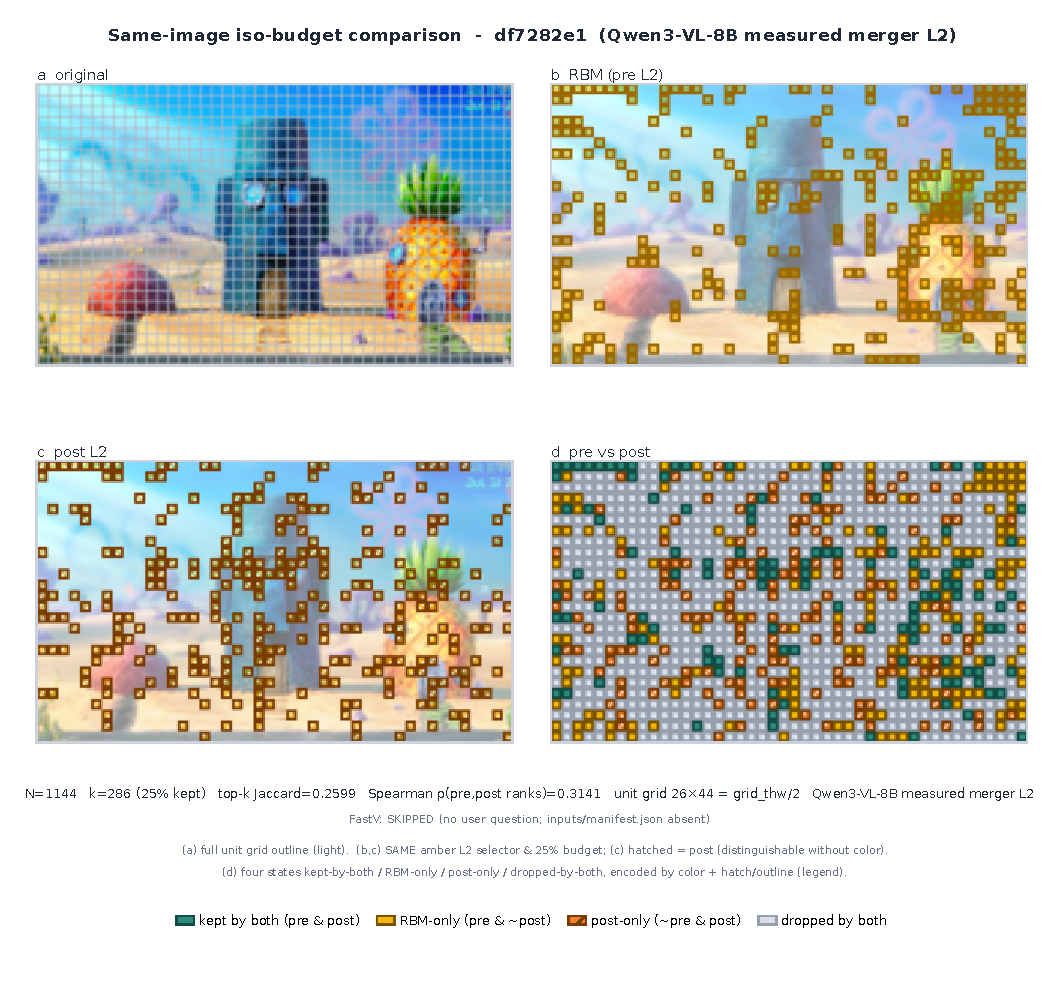
\includegraphics[width=\textwidth]{figs/compare_df7282e1.pdf}
  \caption{Sample \texttt{df7282e1} ($N\!=\!1144$, $k\!=\!286$, $J\!=\!0.260$,
    $\rho\!=\!0.314$). Sparse scene; the four-state map shows RBM-only (amber)
    concentrated on object boundaries while post-only (hatched) scatters over
    flat regions the merger smoothed.}
  \label{fig:cmp_df}
\end{figure*}

\begin{figure*}[p]
  \centering
  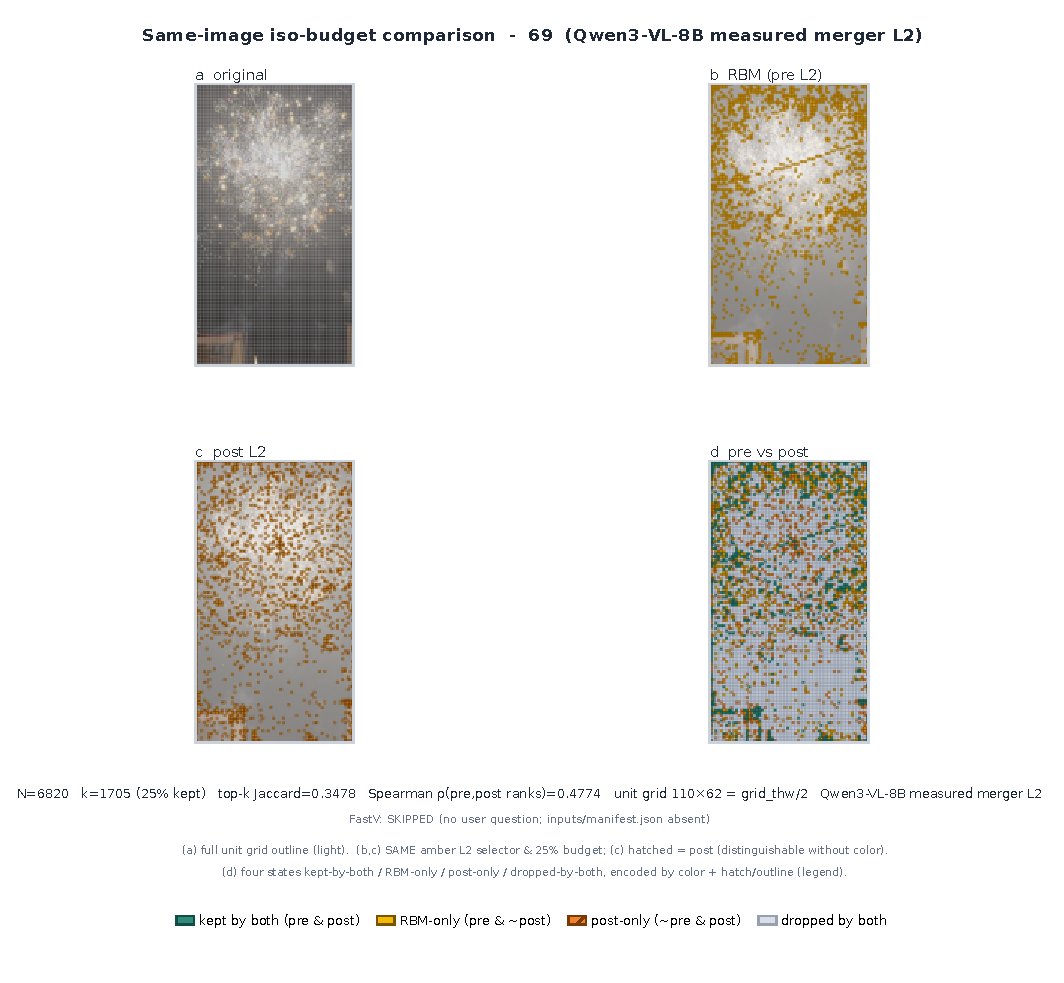
\includegraphics[width=\textwidth]{figs/compare_img69.pdf}
  \caption{Sample \texttt{img69} ($N\!=\!6820$, $k\!=\!1705$, $J\!=\!0.348$,
    $\rho\!=\!0.477$). Highest overlap of the four; the merger preserves more of
    the pre-ranking here, yet two-thirds of the kept set still differs.}
  \label{fig:cmp_69}
\end{figure*}

\begin{figure*}[p]
  \centering
  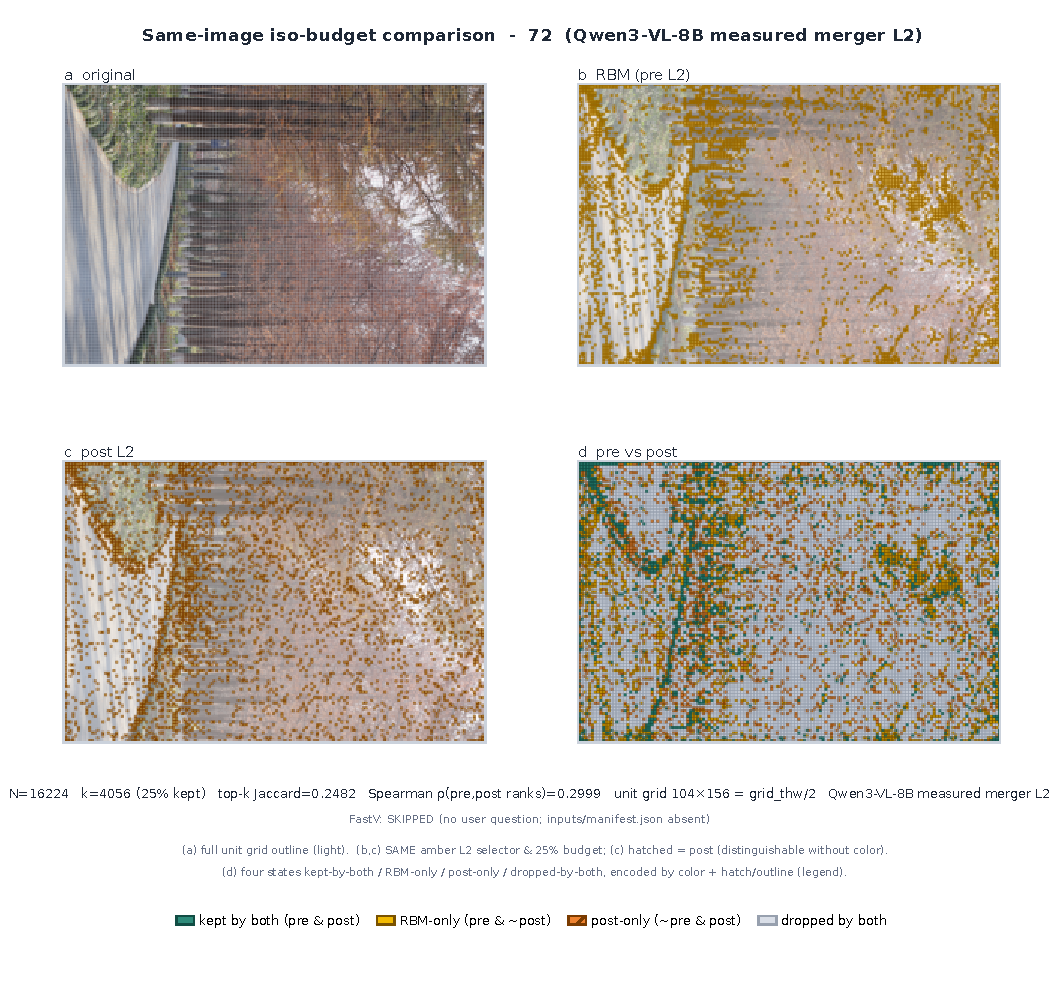
\includegraphics[width=\textwidth]{figs/compare_img72.pdf}
  \caption{Sample \texttt{img72} ($N\!=\!16224$, $k\!=\!4056$, $J\!=\!0.248$,
    $\rho\!=\!0.300$). Textured outdoor scene with a wall edge; the lowest
    overlap --- the merger's lossy aggregation most strongly reorders the
    high-frequency edge vs.\ texture units.}
  \label{fig:cmp_72}
\end{figure*}

\begin{figure*}[p]
  \centering
  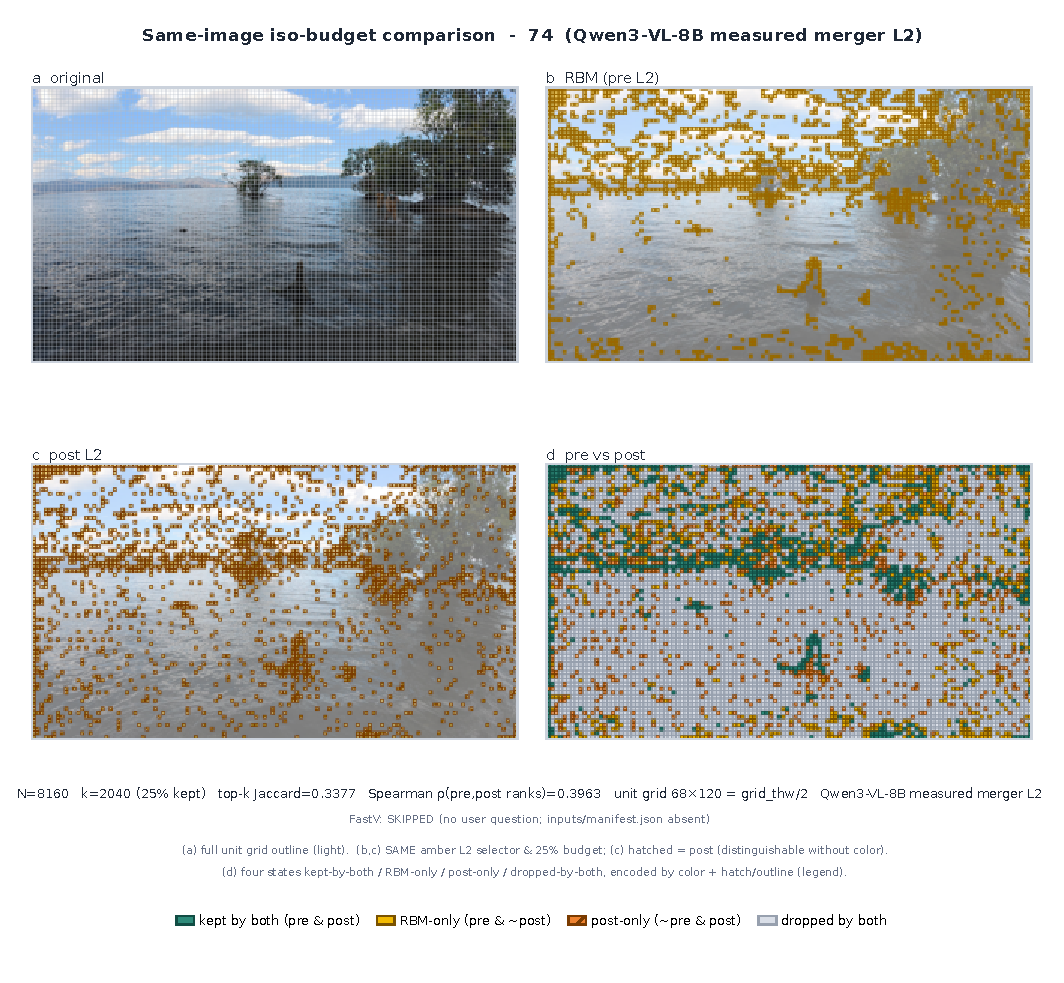
\includegraphics[width=\textwidth]{figs/compare_img74.pdf}
  \caption{Sample \texttt{img74} ($N\!=\!8160$, $k\!=\!2040$, $J\!=\!0.338$,
    $\rho\!=\!0.396$). Waterscape with horizon; RBM-only units track the water
    surface detail that the post-merger L2 demotes in favour of merged sky
    blocks.}
  \label{fig:cmp_74}
\end{figure*}

%──────────────────────────────────────────────────────────────────────────────
\begin{figure*}[p]
\centering
\begin{minipage}{0.86\textwidth}
\section*{S11. Fourth-family gate --- full cell and protocol audit for body Table 2
  (GLM-4.1V-9B-Thinking, $n = 200$)}
\label{app:s11}

This gate tests whether the stage effect transfers to a lineage independent of
Qwen and InternVL. The model uses a GLM-4 text backbone, AIMv2-derived vision
encoder, and a strided $2\!\times\!2$ convolution followed by the
\texttt{Glm4vVisionPatchMerger} MLP. The pre-registered GLM-4.6V-Flash target
could not load because its processor requires transformers $\geq 5.0$rc; the
same-architecture GLM-4.1V fallback was therefore used without a configuration
hack. All nine cells use the same query-blind L2 selector, 25\% retention,
model-default image resolution (effective maximum $\approx 4.82$M pixels),
greedy decoding, and the same thinking-answer parser. Source:
\path{experiments/glm4v_stage_gate.md}; cell JSONs:
\path{runs/glm4v_gate/} (released with code).

\noindent\textbf{Table S11a. Full-precision official scores.}
\begin{center}
  \centering
  \scriptsize
  \begin{tabular}{@{}l l r r r r@{}}
    \toprule
    benchmark & metric & none & pre & post & $\Delta$ (pre$-$post) \\
    \midrule
    TextVQA & VQA-acc     & 0.2417 & 0.2183 & 0.0500 & \textbf{+16.83 pp} \\
    DocVQA  & ANLS        & 0.1039 & 0.1297 & 0.0313 & \textbf{+9.84 pp} \\
    GQA     & exact match & 0.1500 & 0.1600 & 0.1150 & +4.50 pp$^{\dagger}$ \\
    \bottomrule
  \end{tabular}
\end{center}

\noindent\textbf{Table S11b. Token and answer-convergence audit.}
\begin{center}
  \scriptsize
  \begin{tabular}{@{}l r r l@{}}
    \toprule
    benchmark & ptid none & ptid pre/post & boxed none/pre/post \\
    \midrule
    TextVQA & 996.8  & 269.1  & 56/52/15 \\
    DocVQA  & 4868.1 & 1238.8 & 33/30/11 \\
    GQA     & 373.7  & 113.8  & 46/47/39 \\
    \bottomrule
  \end{tabular}
\end{center}

\noindent All cells have $n = 200$ and zero skips. ptid is mean prompt-token
count; pre and post are also exactly equal per sample, not only in the mean.
Boxed counts record samples that reach a final boxed answer within 1024
generated tokens. $^{\dagger}$The GQA direction is protocol-inconclusive and
is not counted as replication.

The prompt-token audit is exact: every paired pre/post example has identical
prompt token ids, and the estimated visual-token counts are approximately
$960\!\to\!233$ (TextVQA), $4830\!\to\!1200$ (DocVQA), and
$347\!\to\!87$ (GQA), with per-image rounding. Thus the large text-dense gaps
cannot be attributed to unequal token budgets. They pass the pre-registered
$5$-pp transfer bar. The other pre-registered half, GQA post$\geq$pre, is not
met: pre exceeds post by 4.5 pp at full $n$, while the $n = 25$ subset where all
three arms reach a boxed answer ties at 0.680/0.680 (pre/post). The latter is a
post-hoc, underpowered diagnostic, not a positive result.

\noindent\textbf{Table S11c. Post-hoc 4096-token diagnostic.}
Cell JSONs: \path{runs/glm4v_gate_v2/} (released with code).
\begin{center}
  \centering
  \scriptsize
  \begin{tabular}{@{}l r r r r r@{}}
    \toprule
    cell & official & contain. & boxed & cut frac. & mean gen. \\
    \midrule
    GQA none     & 0.1650 & 0.290 & 1/200 & 0.740 & 4011 \\
    GQA pre      & 0.1650 & 0.310 & 0/200 & 0.765 & 3997 \\
    GQA post     & 0.1150 & 0.245 & 0/200 & 0.810 & 4057 \\
    TextVQA none & 0.2383 & 0.775 & 2/200 & 0.745 & 3927 \\
    \bottomrule
  \end{tabular}
\end{center}

Increasing max tokens from 1024 to 4096 does not restore greedy convergence:
mean generation remains near the cap and almost no sample reaches a boxed
answer.

The 4096-token probe rules out a short output cap as the source of the GQA
behavior. Its TextVQA containment anchor is $0.775$, close to the published
$\approx 0.77$, while parsed official accuracy remains 0.2383; the model's
visual ability is intact, but deterministic greedy thinking loops rarely
converge to the concise final-answer format. The released model instead
specifies sampling (temperature 0.8, top-$p$ 0.6, top-$k$ 2). We therefore use
this fourth family only as an $n = 200$ replication of the text-dense
pre$\gg$post effect; the full-split claim remains confined to the three model
families in the body, and the GLM GQA direction remains inconclusive.

\par\medskip
\noindent\footnotesize\textbf{Packaging note:} this file converts to the ACM MM
supplementary PDF/archive; run JSONs ship in the code release (anonymous archive
at submission, repository at de-anonymization). Nothing in this supplement
identifies authors, institutions, or repositories (double-blind).
\end{minipage}
\end{figure*}
\clearpage

\end{document}


\end{document}
